% -------------------------------
% Plantilla del TFM en la ESIIAB/ESICR de la UCLM. Versión 0.1 (Preliminar)
%
% Luis de la Ossa
% 
% Compilar con XeLaTeX 
% -------------------------------
\documentclass[12pt, a4paper]{book}

% -------------------------------
% Información y opciones del documento. Debe editarse.
% -------------------------------
% -------------------------------
% Plantilla del TFM en la ESIIAB/ESICR de la UCLM. Versión 0.1 (Preliminar)
%
% Luis de la Ossa
% 
% Compilar con XeLaTeX 
% -------------------------------


% -------------------------------
% Comandos comunes
% -------------------------------
\newcommand{\uclm}{Universidad de Castilla-La Mancha\,}
\newcommand{\dsi}{Departamento de Sistemas Informáticos\,}
\newcommand{\esii}{Escuela Superior de Ingeniería Informática de Albacete\,}
\newcommand{\esi}{Escuela Superior de Informática de Ciudad Real\,}
\newcommand{\iiia}{Instituto de Investigación en Informática de Albacete\,}


% -------------------------------
% Comandos específicos
% -------------------------------
\newcommand{\autor}{Carlos Martínez Jaén\,}
\newcommand{\titulo}{Diseño de una arquitectura lakehouse escalable para la integración y análisis de información curricular académica\,}
\newcommand{\director}{Luis De La Ossa Jiménez\,}
% Sin codirector.
\newcommand{\fecha}{Octubre, 2026\,}
\newcommand{\espec}{Máster en Big Data y Computación en la Nube\,}







% -------------------------------
% Configuración del documento, paquetes, etc. 
% -------------------------------
% -------------------------------
% Plantilla del TFM en la ESIIAB/ESICR de la UCLM. Versión 0.1 (Preliminar)
%
% Luis de la Ossa
% 
% Compilar con XeLaTeX 
% -------------------------------


% -------------------------------
% Idioma
% -------------------------------
\usepackage{polyglossia}
\setmainlanguage{spanish}


% -------------------------------
% Fuente
% -------------------------------
% Cualquier tamaño de texto: {\fontsize{100pt}{120pt}\selectfont tutexto}
\usepackage{anyfontsize}
% Selección de fuentes.
\usepackage{fontspec}
% Espacio entre líneas
\usepackage{setspace}
% Fuentes especiales
\usepackage{textcomp,marvosym,pifont}


% -------------------------------
% Otros paquetes de uso común
% -------------------------------
% Símbolos matemáticos
\usepackage{amsmath,amsfonts,amssymb}
% Gráficos
\usepackage{graphicx}
% Posición arbitraria de los gráficos
\usepackage[absolute,overlay]{textpos}
% Apéndices
\usepackage{appendix}


% -------------------------------
% Esquema de colores
% -------------------------------
% Paquete para la definición de colores
\usepackage[table]{xcolor}
% Esquema de colores
% -------------------------------
% Plantilla del TFM en la ESIIAB/ESICR de la UCLM. Versión 0.1 (Preliminar)
%
% Luis de la Ossa
% 
% Compilar con XeLaTeX 
% -------------------------------

% -------------------------------
% Color del tema
% -------------------------------

% Color para los títulos, etc.
%\definecolor{tema}{RGB}{0,0,0}            % Negro (Recomendado)
%\definecolor{tema}{gray}{.50}            % Gris 50
%\definecolor{tema}{RGB}{183, 18, 52}     % LOGO UCLM
\definecolor{tema}{RGB}{0, 69, 134}       % Azul del esquema (mismo tono que la memoria del TFG)
%\definecolor{tema}{RGB}{153, 61, 61}     % Rojo del esquema

% Negritas con el color del tema
\newcommand{\bft}[1]{\textcolor{tema}{\bf #1}} 


% -------------------------------
% Esquema de colores
% -------------------------------
% Se pueden redefinir para que coincidan con las paletas de las 
% herramientas utilizadas para hacer las gráficas.
\definecolor{blanco}{RGB}{255,255,255} 
\definecolor{negro}{RGB}{0,0,0}
\definecolor{gris95}{gray}{.95}
\definecolor{gris75}{gray}{.75}
\definecolor{gris50}{gray}{.50}
\definecolor{gris25}{gray}{.25}
\definecolor{rojo}{RGB}{153, 61, 61}        
\definecolor{uclm}{RGB}{183, 18, 52}       % Corporativo UCLM
\definecolor{azul}{RGB}{31, 78, 121}       
\definecolor{verde}{RGB}{82, 112, 87}      
\definecolor{naranja}{RGB}{196, 118, 58} 
\definecolor{mostaza}{RGB}{179, 147, 63} 

% Negrita con color definido 
\newcommand{\bfa}[1]{\textcolor{azul}{\bf #1}} 
\newcommand{\bfr}[1]{\textcolor{rojo}{\bf #1}}
\newcommand{\bfn}[1]{\textcolor{naranja}{\bf #1}}
\newcommand{\bfv}[1]{\textcolor{verde}{\bf #1}}  
\newcommand{\bfm}[1]{\textcolor{mostaza}{\bf #1}} 






% -------------------------------
% Márgenes
% -------------------------------
% Márgenes de las páginas
\usepackage[
  inner	 =	3cm,   % Margen interior
  outer	 =	2.5cm, % Margen exterior
  top	 =	2.5cm, % Margen superior
  bottom =	2.5cm, % Margen inferior
  includeheadfoot, % Incluye cabecera y pie de página en los márgenes
]{geometry}

% Muestra una regla para comprobar el formato de las páginas (descomentar)
%\usepackage[type=upperleft,showframe,marklength=8mm]{fgruler} 


% -------------------------------
% Interlineado
% -------------------------------
\usepackage{setspace}
\onehalfspacing    % interlineado 1.5
%\doublespacing     % interlineado doble
%\singlespacing     % normal


% -------------------------------
% Líneas viudas y huérfanas
% -------------------------------
% Evita que quede una única línea de un párrafo suelta al principio o al
% final de una página (línea viuda/huérfana).
\clubpenalty=10000
\widowpenalty=10000
\displaywidowpenalty=10000
% Permite que una página termine algo antes del margen inferior en vez de
% estirar el espacio entre párrafos para rellenarla (\flushbottom, el
% comportamiento por defecto en "twoside", produce huecos verticales muy
% visibles al combinarse con la restricción anterior).
\raggedbottom


% -------------------------------
% Renombra tablas y bibliografía
% -------------------------------
\addto\captionsspanish{
	\renewcommand{\listtablename}{Índice de tablas} 
	\renewcommand{\tablename}{Tabla}
	\renewcommand{\bibname}{Referencia bibliográfica}
}


% -------------------------------
% Itemize y enumerate. Control de los espacios.
% -------------------------------
\usepackage{enumitem}
\setitemize{itemsep=0pt}
\setenumerate{itemsep=0pt}
\renewcommand{\labelitemi}{\tiny\bft{$\blacksquare$}}
\renewcommand{\labelitemii}{\bft{$\bullet$}}
\renewcommand{\labelitemiii}{\bft{-}}


% -------------------------------
% Enlaces y colores
% -------------------------------
\usepackage{hyperref}
%\hypersetup{
%    colorlinks,
%    citecolor=black,
%    filecolor=black,
%    linkcolor=black,
%    urlcolor=black
%}

% -------------------------------
% Evita títulos de sección huérfanos
% -------------------------------
% Permite \needspace{...} justo antes de un \section para forzar el salto
% de página antes del título, en vez de después (evita que un título quede
% solo al final de una página con su contenido -- p. ej. una tabla [H] --
% en la página siguiente).
\usepackage{needspace}

% -------------------------------
% Gestión de elementos flotantes
% -------------------------------
% Para forzar a que las figuras y tablas aparezcan antes del fin de una
% sección, en vez de derivar hacia la siguiente (evita que una tabla
% termine flotando en medio de la sección siguiente).
\usepackage[section]{placeins}
% Permite el especificador [H] (posición exacta) para tablas/figuras
% cortas referenciadas inmediatamente en el texto, evitando que floten
% varias páginas más allá de su primera mención.
\usepackage{float}

% -------------------------------
% Diagramas nativos, para figuras de arquitectura y flujo dibujadas
% directamente en LaTeX, sin depender de un renderizador externo
% -------------------------------
\usepackage{tikz}
\usetikzlibrary{positioning,arrows.meta,shapes.geometric,calc}

% Gestión de títulos de los elementos flotantes
\usepackage{caption}
% Subfiguras y títulos en subfiguras
\usepackage{subcaption}

% Títulos
\DeclareCaptionFont{tema}{\color{tema}} % Color
\captionsetup{labelfont={tema, bf}}     % Estilo
\captionsetup{font=normalsize}          % Tamaño
\captionsetup{width=.9\linewidth}       % Anchura del título
 % Distancia de la figura al texto.
\setlength{\intextsep}{1cm} 
\setlength{\textfloatsep}{1cm}         
       

% -------------------------------
% Utilidades para tablas
% -------------------------------
% Para fundir filas en tablas
\usepackage{multirow}
% Para definir columnas con ancho fijo y alineación
\usepackage{array,ragged2e}
\newcolumntype{L}[1]{>{\raggedright\let\newline\\\arraybackslash\hspace{0pt}}m{#1}}
\newcolumntype{C}[1]{>{\centering\let\newline\\\arraybackslash\hspace{0pt}}m{#1}}
\newcolumntype{R}[1]{>{\raggedleft\let\newline\\\arraybackslash\hspace{0pt}}m{#1}}


% -------------------------------
% Para tabular
% -------------------------------
\usepackage{tabto}


% -------------------------------
% Formato de títulos, capítulos, etc.
% -------------------------------
\usepackage{titlesec, titletoc}
% Parte
\titleformat{\part}[display]												     	   % Estilo
	{\Huge \centering \color{tema}}                                                % Formato
	{Parte \thepart }                                                              % Etiqueta
	{0.75ex}                                                                       % Separación
	{\bfseries\fontsize{25pt}{40pt}\selectfont}                                    % Entre etiqueta y título            
	[\thispagestyle{empty}]                                                        % Después

% Capítulo		
\titleformat{\chapter}[block]            			 			                    % Estilo  	
	{\vspace{0cm} \flushright \bfseries \LARGE \color{tema}}  	        		% Formato 
	{\thechapter.}                  			  									% Etiqueta
	{0.75ex}                                     									% Separación
	{}                                           									% Entre etiqueta y título
	[\vspace{-0.25cm} \rule{0.5\textwidth}{1pt}\vspace*{1cm}\thispagestyle{plain}]    % Después      
  
% Sección
\titleformat{\section}
	{\vspace{5pt}  \Large \color{tema}}
	{\thesection .}
	{0.75ex}
	{}

% Subsección
\titleformat{\subsection}
	{\large \color{tema}}
	{\thesubsection .}
	{0.75ex}
	{}
 
% Subsubsección
\titleformat{\subsubsection}
	{\bf\color{tema}}
	{}
	{0.75ex}
	{}
	 
% Parte (TOC)
\titlecontents{part}[2pc]
  	{\vspace{20pt}\bfseries\filright\Large\color{tema}}
  	{\contentslabel{1.5pc}}{\hspace*{-1.5pc}}
  	{\vspace{5pt}}
  	{}
  
% Capítulo (TOC)
\titlecontents{chapter}[2pc]
  	{\vspace{10pt}\bfseries\large\filright}
  	{\contentslabel{1.5pc}}{\hspace*{-1.5pc}}
  	{\mdseries\titlerule*[0.5pc]{.}\bfseries\contentspage}

% Sección (TOC)
\titlecontents{section}[4pc]
  	{\vspace{5pt}\filright}
  	{\contentslabel{2pc}}{\hspace*{2pc}}
  	{\titlerule*[0.5pc]{.}\contentspage}
  	{\vspace{5pt}}

% Subsección (TOC)
\titlecontents{subsection}[6pc]
  	{\vspace{2.5pt}\filright\small\em}
  	{\contentslabel{3pc}}{\hspace*{-3pc}}
  	{\titlerule*[0.5pc]{.}\contentspage} 
  	
  	
% -------------------------------
% Cabeceras y pie de página
% -------------------------------
\usepackage{fancyhdr}
\pagestyle{fancy}
\fancyhf{}

% Permite incluir la parte. Para ello crea \parttitle
\let\Oldpart\part
\newcommand{\parttitle}{}
\renewcommand{\part}[1]{\Oldpart{#1}\renewcommand{\parttitle}{#1}}

% Cabeceras y pies de página
\fancyhead[LE]{}
\fancyhead[RO]{\slshape \leftmark}
\fancyfoot[LE,RO]{\thepage}
\renewcommand{\footrulewidth}{1pt}
\renewcommand{\headrulewidth}{1pt}
\renewcommand{\chaptermark}[1]{\markboth{#1}{}} % Capítulo (Solo texto)
\renewcommand{\chaptermark}[1]{\markboth{\thechapter. #1}{}} % Capítulo (Número y texto)

% Formato plano para las páginas con títulos (solo incluye el pie de página)
\fancypagestyle{plain}{
\fancyhf{}
\fancyhead{}
\fancyfoot[LE,RO]{\thepage}
\renewcommand{\footrulewidth}{1pt}
\renewcommand{\headrulewidth}{0pt}
}

 
% -------------------------------
% Utilidades
% -------------------------------
% Marcas
\newcommand{\pcite}{\bfr{\large[?]}\,} % Cita pendiente: [?] en rojo y negrita.
\newcommand{\ps}{\bfr{\huge[--}\,} % Pricipio de un bloque en sucio
\newcommand{\fs}{\bfr{\huge--]}\,} % Fin de un bloque en sucio.

% Notas
\usepackage[textsize=tiny,spanish,shadow,textwidth=2cm]{todonotes}

% Para generar textos "random"
\usepackage{lipsum} 
 

% -------------------------------
% Algoritmos y código
% -------------------------------

% Se definen entornos específicos para algoritmos y código que permiten
% gestionar los títulos manera similar en ambos casos, y similar al resto
% de elementos flotantes.
\usepackage{newfloat}

\DeclareFloatingEnvironment[ % Algoritmos
  listname = {Índice de algoritmos},
  name = Algoritmo
]{algorithm}

\DeclareFloatingEnvironment[ % Fragmentos de código
  listname = {Índice de listados de código},
  name = Código
]{code}

% Define un estilo para el encabezado de algoritmos y código.
\DeclareCaptionFormat{algcode}{
% OPCIÓN 1 -> Línea debajo del título
%{\color{gris50}\rule{\dimexpr\textwidth\relax}{0.4pt}\vspace{0cm}}
%#1#2#3
%\vspace{-0.2cm}{\color{gris50}\rule{\dimexpr\textwidth\relax}{0.4pt}} % 
% OPCIÓN 2 -> Sin línea debajo del título
{\color{gris50}\rule{\textwidth}{0.4pt}\vspace{0cm}}
#1#2#3
}
\captionsetup[algorithm]{format=algcode, width=\linewidth}
\captionsetup[code]{format=algcode, width=\linewidth}

% Opciones específicas para algoritmos.
\usepackage[noend]{algpseudocode}
% Tamaño de letra y separadores
\makeatletter
\renewcommand{\ALG@beginalgorithmic}{{\color{gris50}\small\hrule\vskip10pt}}
\makeatother
% Variables y funciones
\newcommand{\va}[1]{{\it {#1}}}				
\newcommand{\fu}[1]{{\textsc{#1}}}          
% Palabras clave
\renewcommand{\algorithmicrepeat}{\bft{repetir}}
\renewcommand{\algorithmicuntil}{\bft{hasta}}
\renewcommand{\algorithmicend}{\bft{fin}}
\renewcommand{\algorithmicif}{\bft{si}}
\renewcommand{\algorithmicthen}{\bft{entonces}}
\renewcommand{\algorithmicelse}{\bft{si no}}
\newcommand{\algorithmicelsif}{\algorithmicelse\ \algorithmicif}
\newcommand{\algorithmicendif}{\algorithmicend\ \algorithmicif}
\renewcommand{\algorithmicfor}{\bft{para}}
\renewcommand{\algorithmicforall}{\bft{para cada}}
\renewcommand{\algorithmicwhile}{\bft{mientras}}
\renewcommand{\algorithmicdo}{\bft{hacer}}
\renewcommand{\algorithmicprocedure}{\bft{procedimiento}}
\renewcommand{\algorithmicreturn}{\bft{devolver}}
\renewcommand{\algorithmicfunction}{\bft{función}}
\renewcommand{\algorithmicloop}{\bft{iterar}}

% Opciones específicas para código.
\usepackage{listings}
% Aspecto de los listados de código (ejemplo)
% Los colores se han de cambiar y adaptar a los distintos lenguajes de programación.
\lstset{
    language=Python,
    keywordstyle=\bf\color{tema},  
	breaklines=true,    
	basicstyle={\small\ttfamily},
    tabsize=5,
    rulecolor=\color{gray!50},
    frame=t % Es importante no cambiar esta opción (es la línea superior) 
}

% -------------------------------
% Cacacteres pifont de uso común (con color)
% -------------------------------
\newcommand{\vmarkt}{\textcolor{tema}{\ding{52}} }  % Checked (V) Tema
\newcommand{\vmarkr}{\textcolor{rojo}{\ding{52}} }  % Checked (V) Rojo
\newcommand{\vmarka}{\textcolor{azul}{\ding{52}} }  % Checked (V) Azul

\newcommand{\xmarkt}{\textcolor{tema}{\ding{55}} }  % Checked (X) Tema
\newcommand{\xmarkr}{\textcolor{rojo}{\ding{55}} }  % Checked (X) Rojo
\newcommand{\xmarka}{\textcolor{azul}{\ding{55}} }  % Checked (X) Azul

\newcommand{\lmarkt}{\textcolor{tema}{\ding{46}} }  % Lápiz Tema
\newcommand{\lmarkr}{\textcolor{rojo}{\ding{46}} }  % Lápiz Rojo
\newcommand{\lmarka}{\textcolor{azul}{\ding{46}} }  % Lápiz Azul

\newcommand{\hmarkt}{\textcolor{tema}{\ding{43}} }  % Mano Tema
\newcommand{\hmarkr}{\textcolor{rojo}{\ding{43}} }  % Mano Roja 
\newcommand{\hmarka}{\textcolor{azul}{\ding{43}} }  % Mano Azula 

\newcommand{\fmarkt}{\textcolor{tema}{\ding{220}} }  % Flechza Tema
\newcommand{\fmarkr}{\textcolor{rojo}{\ding{220}} }  % Flecha Roja 
\newcommand{\fmarka}{\textcolor{azul}{\ding{220}} }  % Flecha Azul

% Documento
\begin{document}

% -------------------------------
% Portada y título
% -------------------------------
% Fuente  de la portada
% \setmainfont[Ligatures={NoRequired,NoCommon,NoContextual}]{Calibri}
% -------------------------------
% Plantilla del TFM en la ESIIAB/ESICR de la UCLM. Versión 0.1 (Preliminar)
%
% Luis de la Ossa
% 
% Compilar con XeLaTeX 
% -------------------------------
\pagestyle{empty}
\begin{titlepage}\null



\begin{textblock*}{\paperwidth}(0cm,2.5cm)
\begin{center}

\includegraphics[width=4cm]{figs/logoconciti.png}
\end{center}
\end{textblock*}


\begin{textblock*}{\paperwidth}(0cm,7.5cm) 
\begin{center}\doublespacing
{\fontsize{18pt}{2pt}\selectfont \uclm}

\vspace*{0.2cm}
{\fontsize{16pt}{2pt}\selectfont \esii}

{\fontsize{16pt}{2pt}\selectfont \esi}
\end{center}
\end{textblock*}


\begin{textblock*}{\paperwidth}(0cm,12.5cm) 
\begin{center}\doublespacing 
{\bf\fontsize{18pt}{4pt}\selectfont Trabajo Fin de Máster}

\vspace*{0.2cm}
{\fontsize{18pt}{4pt}\selectfont \espec}

\end{center}
\end{textblock*}



\begin{textblock*}{\textwidth}(3cm, 17.5cm) 
\begin{center}\doublespacing % onehalfspace
{\bf\fontsize{20pt}{4pt}\selectfont \titulo}

\vskip1cm
{\it \fontsize{18pt}{4pt}\selectfont \autor}
\end{center}
\end{textblock*}


\begin{textblock*}{\textwidth}(3cm,25.25cm) 
\begin{center}
{\fontsize{14pt}{4pt}\selectfont \fecha}
\end{center}
\end{textblock*}
\end{titlepage}

% -------------------------------
% Fuente del documento.
% -------------------------------
% Calibri (fuente por defecto de la plantilla) es una fuente propietaria de
% Microsoft, no disponible en Linux; se usa la misma alternativa libre que
% adoptó el TFG.
\setmainfont{TeX Gyre Termes}

% -------------------------------
% Preámbulo
% -------------------------------
\frontmatter 
% -------------------------------
% Plantilla del TFM en la ESIIAB/ESICR de la UCLM. Versión 0.1 (Preliminar)
%
% Luis de la Ossa
% 
% Compilar con XeLaTeX 
% -------------------------------


% -------------------------------
% Segunda portada
% -------------------------------
\cleardoublepage
\setcounter{page}{1} \null


\begin{textblock*}{3cm}(15cm,23cm) 
\begin{center}

\includegraphics[height=1.2cm]{figs/logouclm.jpg}
\end{center}
\end{textblock*}



\begin{textblock*}{\textwidth}(2.8cm,2.6cm)  % Corrige la posición 
\begin{flushleft}

\includegraphics[height=0.8cm]{figs/logoesii.png} 
\end{flushleft}
\end{textblock*}

\begin{textblock*}{\textwidth}(3cm,2.37cm)  % Corrige la posición
\begin{flushright}

\includegraphics[height=1cm]{figs/logoesi.png} 
\end{flushright}
\end{textblock*}

\begin{textblock*}{\textwidth}(3cm,6.5cm) 
\begin{center}\doublespacing 
{\fontsize{18pt}{4pt}\selectfont \bft{TRABAJO FIN DE MÁSTER}}

\medskip
{\fontsize{18pt}{4pt}\selectfont \espec}


\end{center}
\end{textblock*}


\begin{textblock*}{\textwidth}(3cm,12.5cm) 
\begin{center}\doublespacing 
{\fontsize{22pt}{4pt}\selectfont \bft{\titulo}}
\end{center}
\end{textblock*}


\begin{textblock*}{\textwidth}(3cm, 19.5cm) 
\begin{flushleft}\doublespacing
{\fontsize{14pt}{4pt}\selectfont \bft{Autor:} \autor}

{\fontsize{14pt}{4pt}\selectfont \bft{Director:} \director}
\end{flushleft}
\end{textblock*}


\begin{textblock*}{\textwidth}(3cm,24.75cm) 
\begin{flushright}
{\fontsize{14pt}{4pt}\selectfont \fecha}
\end{flushright}
\end{textblock*}


% -------------------------------
% Dedicatoria
% -------------------------------
\cleardoublepage
\thispagestyle{empty}

\vspace*{9cm}  
\begin{flushright} \em 
Aquí va la dedicatoria que cada cual \\ 
quiera escribir. El ancho se controla \\ 
manualmente
\end{flushright}


% -------------------------------
% Declaración de autoría
% -------------------------------
\cleardoublepage
\thispagestyle{plain}
\chapter*{Declaración de autoría}

%\begin{center}
%\Large{\bft{Declaración de autoría}}
%\end{center}
%\vskip1cm

Yo, \autor, con DNI \quad \dniautor \quad, declaro que soy el único autor del trabajo fin de máster titulado ``\titulo'', que el citado trabajo no infringe las leyes en vigor sobre propiedad intelectual, y que todo el material no original contenido en dicho trabajo está apropiadamente atribuido a sus legítimos autores.

\vspace*{2cm}
\begin{center}
Albacete, a \quad \ldots \quad de \quad \ldots \quad de 20 \ldots

\vskip3cm

Fdo.: \autor
\end{center}


% -------------------------------
% Resumen
% -------------------------------
\cleardoublepage
\thispagestyle{plain}
\chapter*{Resumen}
%\begin{center}
%\Large{\bft{Resumen}}
%\end{center}
%\vskip0.5cm

La información curricular y de trayectoria investigadora se reparte entre
documentos individuales, como los currículos CVN, y registros públicos a
escala masiva, como los perfiles de ORCID. Los sistemas de información de
investigación interoperan datos de este tipo sobre infraestructura
institucional cerrada, y no existe una plataforma abierta, autoalojada y
reproducible que combine ambas naturalezas de dato y las procese de forma
conjunta.

Este Trabajo Fin de Máster diseña, despliega y evalúa una plataforma
\textit{lakehouse} que integra ORCID real con CVN sintético y publica
indicadores de investigación. La plataforma se despliega sobre Kubernetes y
combina almacenamiento de objetos con Iceberg, procesamiento distribuido con
Spark, orquestación con Airflow, publicación en PostgreSQL y visualización
con Superset. Los currículos CVN se generan de forma sintética, válidos
frente al formato Open CVN y sembrados con campos públicos de ORCID, de modo
que no se tratan datos personales de terceros. Esa siembra enlaza cada
currículo con su perfil real y sirve de base a una resolución de identidad
determinista, con evidencia explícita en cada fusión.

La evaluación usa datos reales. Sobre más de 26 millones de registros de
ORCID se filtraron 301\,763 perfiles con afiliación española, y la
resolución de identidad alcanzó una precisión del 95,8\% y una cobertura del
74,2\% en su regla de repliegue por nombre y afiliación. Un banco de pruebas
de rendimiento sobre tres volúmenes de datos demuestra que el número de
ejecutores de Spark es una palanca de fiabilidad, no solo de velocidad: con
la memoria fija por ejecutor, un único ejecutor deja de completar la
transformación a partir del doble del volumen base. Por último, la
plataforma completa se reconstruyó desde cero sobre un clúster aislado
siguiendo únicamente una guía escrita, lo que confirma su reproducibilidad.

% -------------------------------
% Agradecimientos
% -------------------------------
\cleardoublepage
\thispagestyle{plain}
\vspace*{4cm}
\begin{center}
\Large{\bft{Agradecimientos}}
\end{center}
\vskip0.5cm

\lipsum[1]

% -------------------------------
% Índices y tablas
% -------------------------------
% Cambia a interlineado normal
\singlespacing     

\tableofcontents	% Índice
\listoffigures		% Índice de figuras
\listoftables		% Índice de tablas
\listofalgorithms   % Índice de algoritmos (comentar si no los hay)
\listofcodes	    % Índice de códigos (comentar si no los hay)
\cleardoublepage

% Vuelve a interlineado de 1.5
\onehalfspacing 

% -------------------------------
% Documento
% -------------------------------
\mainmatter
% Estilo de página
\pagestyle{fancy}


% Introducción, motivación y objetivos
\chapter{Introducción, motivación y objetivos}
\label{cap:introduccion}

El presente capítulo introduce el contexto en el que se enmarca este
Trabajo Fin de Máster, en adelante TFM, describe la motivación que
justifica su desarrollo y delimita los objetivos que guían la solución
propuesta. Para ello, en primer lugar se sitúa el trabajo con respecto al
Trabajo Fin de Grado, en adelante TFG, previo del mismo autor, del que
parte directamente. A continuación, se expone el problema de partida y la
motivación que lo sustenta, se establecen los objetivos general y
específicos, se recogen los aspectos éticos y de privacidad que afectan al
tratamiento de los datos empleados y se relacionan los objetivos con los
resultados de aprendizaje del máster. Finalmente, se presenta la
estructura seguida por el resto del documento.

\section{Contexto y continuidad con el Trabajo Fin de Grado}
\label{sec:introduccion_contexto}

Este TFM se construye directamente sobre el trabajo ya cerrado y defendido
en el TFG del mismo autor~\cite{tfg_open_cvn}, del que hereda el punto de
partida técnico: una capa estructural reproducible generada a partir de
los esquemas oficiales de CVN, una normalización trazable de sus
metadatos, y un formato abierto, validable y extensible, Open CVN JSON,
con su propio contrato de parseo y validación.

El presente trabajo reutiliza ese resultado como una de sus dos fuentes de
datos, no como objeto de estudio: se reutilizan directamente el esquema
JSON Schema de Open CVN, su contrato de validación ya implementado, y las
convenciones de trazabilidad de procedencia, en inglés
\textit{provenance}, establecidas en la capa semántica del TFG. Por ello,
este documento no vuelve a definir qué es CVN ni qué es Open CVN,
remitiendo esa exposición al TFG anterior, y se limita a describir cómo
dicho formato, ya cerrado, se ingiere, valida y procesa dentro de la
plataforma distribuida que aquí se construye.

Este cambio de perspectiva, de un formato y una herramienta de un único
usuario a una plataforma que ingiere, fusiona y procesa datos a escala,
responde también a un cambio de programa académico. Mientras que el TFG se
enmarcaba en la intensificación de Computación, este TFM pertenece al
Máster en Big Data y Computación en la Nube, cuyos resultados de
aprendizaje se detallan en la Sección~\ref{sec:introduccion_outcomes}.

\section{Problema de partida y motivación}
\label{sec:introduccion_motivacion}

La información curricular y de trayectoria investigadora se encuentra
dispersa en fuentes heterogéneas, de distinta naturaleza y de distinto
volumen. Por un lado, documentos curriculares como CVN describen la
actividad de un investigador de forma estructurada pero unitaria, pensada
para su presentación individual ante convocatorias, evaluaciones o
acreditaciones. Por otro lado, registros públicos como los perfiles de
ORCID, siglas en inglés de \textit{Open Researcher and Contributor
ID}~\cite{orcid_about}, agregan identificadores, filiaciones y producción
científica de investigadores de todo el mundo a escala global. Solo el
fichero público de datos de ORCID de 2025 reúne más de 26 millones de
registros~\cite{orcid_public_data_file_2025}.

Los sistemas de información de investigación, conocidos por sus siglas en
inglés como CRIS, de \textit{Current Research Information Systems},
interoperan datos de este tipo entre instituciones mediante modelos
comunes como CERIF~\cite{eurocris_cerif} o plataformas como
VIVO~\cite{vivo_project}. Sin embargo, lo hacen sobre infraestructura
institucional cerrada, sin publicar una plataforma de referencia abierta,
autoalojada y reproducible que combine específicamente currículos
normalizados como CVN con perfiles públicos como ORCID. Estas dos
naturalezas de dato, documental y de registro masivo público, rara vez se
integran, procesan conjuntamente y publican como indicadores agregados
dentro de una misma plataforma de este tipo.

Esta ausencia responde a un problema de arquitectura. Integrar fuentes de
esta naturaleza exige:

\begin{itemize}
  \item \textbf{Almacenamiento escalable}, capaz de crecer con el volumen
  real de ORCID.
  \item \textbf{Un formato de tabla que preserve evolución de esquema y
  trazabilidad}, dado que CVN y ORCID no comparten esquema.
  \item \textbf{Procesamiento distribuido tolerante a fallos}, para
  transformar ese volumen en un tiempo razonable.
  \item \textbf{Orquestación de flujos de trabajo}, que encadene ingesta,
  transformación y publicación de forma reproducible.
  \item \textbf{Una capa de resolución de identidad}, capaz de fusionar
  registros de fuentes distintas que describen a la misma persona.
\end{itemize}

Ninguno de estos elementos formaba parte del alcance del TFG, centrado
deliberadamente en un único documento curricular.

La motivación de este trabajo consiste, por tanto, en demostrar, mediante
una plataforma real desplegada y no mediante un diseño exclusivamente
documental, las competencias propias de un perfil de Big Data y
Computación en la Nube:

\begin{itemize}
  \item Levantar infraestructura distribuida.
  \item Ingerir y fusionar fuentes heterogéneas.
  \item Procesar los datos a escala con tolerancia a fallos.
  \item Evaluar el sistema con datos y cifras reales obtenidos de su
  propia ejecución, en lugar de resultados simulados o proyectados.
\end{itemize}

\section{Objetivos}
\label{sec:introduccion_objetivos}

El objetivo general de este Trabajo Fin de Máster es \textit{diseñar,
desplegar y evaluar una plataforma que integre datos curriculares de CVN
sintético y datos de investigación de ORCID real, los procese de forma
distribuida con resolución de identidad entre fuentes, y publique un
conjunto reducido de indicadores de investigación en un panel de
visualización, evaluando el sistema mediante un \textit{benchmark} de
rendimiento acotado}. Los objetivos que siguen se formulan de forma
agnóstica respecto a la arquitectura y las tecnologías concretas que los
satisfacen. Esa elección se presenta y se justifica frente a sus
alternativas en el Capítulo~\ref{cap:estado_arte}.

Para alcanzar esta meta global se han definido los siguientes objetivos
específicos:

\begin{enumerate}
  \item \textbf{Desplegar la infraestructura base de la plataforma.}
  Comprende la puesta en marcha del entorno de cómputo y de los servicios
  de almacenamiento, persistencia y orquestación sobre los que se apoya el
  resto del sistema.

  \item \textbf{Validar el mecanismo central de almacenamiento y
  procesamiento distribuido.} Antes de construir cualquier flujo de datos
  de negocio sobre la plataforma, se comprueba de forma aislada que dicho
  mecanismo funciona de extremo a extremo.

  \item \textbf{Incorporar datos ORCID reales a la plataforma.} Combina el
  enriquecimiento puntual de registros concretos con la incorporación de un
  volumen real de datos, ambos obtenidos de fuentes públicas de ORCID.

  \item \textbf{Incorporar currículos CVN a la plataforma, validados frente
  al formato Open CVN.} Estos currículos se obtienen por generación
  sintética a partir de datos públicos, no por recolección de currículos
  reales, tal y como se justifica en la Sección~\ref{sec:introduccion_etica}.

  \item \textbf{Integrar los datos de ORCID con los datos CVN por medio del
  formato Open CVN, resolviendo la identidad de los registros que
  corresponden a la misma persona.} Constituye la fusión efectiva entre las
  dos fuentes de datos del sistema.

  \item \textbf{Calcular indicadores de investigación agregados y
  publicarlos de forma consistente.} Los indicadores deben quedar
  disponibles para su consumo posterior sin estados intermedios ni
  publicaciones parciales.

  \item \textbf{Visualizar los indicadores publicados en un panel
  accesible.} Permite comprobar que los indicadores calculados son
  consumibles más allá del propio sistema que los produce.

  \item \textbf{Medir el efecto del grado de paralelismo del procesamiento
  distribuido sobre el tiempo de ejecución y la fiabilidad, a distintas
  escalas de datos.} Constituye el \textit{benchmark} de rendimiento
  acotado exigido por el planteamiento del proyecto.

  \item \textbf{Encontrar y corregir defectos de robustez operativa mediante
  el uso real del sistema completo.} Este objetivo, sin equivalente directo
  en el TFG anterior, exige documentar una guía de reproducción del entorno
  desde cero y registrar los fallos de infraestructura detectados y
  corregidos como parte de la evaluación del sistema.
\end{enumerate}

La Tabla~\ref{tab:tfm_objetivos_capitulos} relaciona estos objetivos con
los capítulos principales en los que se desarrollan. Es en esos capítulos,
no aquí, donde cada objetivo se concreta en una arquitectura y unas
tecnologías determinadas.

\begin{table}[htbp]
  \centering
  \renewcommand{\arraystretch}{1.2}
  \begin{tabular}{p{0.12\textwidth} p{0.58\textwidth} p{0.18\textwidth}}
    \hline
    \textbf{Objetivo} & \textbf{Descripción resumida} & \textbf{Capítulos} \\
    \hline
    OE1 & Despliegue de la infraestructura base de la plataforma & 3 \\
    OE2 & Validación del mecanismo central de almacenamiento y procesamiento & 3 \\
    OE3 & Incorporación de datos ORCID reales & 4 \\
    OE4 & Incorporación de currículos CVN, validados frente a Open CVN & 4 \\
    OE5 & Integración de ORCID con CVN por medio de Open CVN & 5 \\
    OE6 & Cálculo y publicación consistente de indicadores & 5 \\
    OE7 & Visualización de los indicadores en un panel accesible & 6 \\
    OE8 & Benchmark de rendimiento por grado de paralelismo y escala de datos & 6 \\
    OE9 & Robustez operativa mediante uso real y guía de reproducción & 6 \\
    \hline
  \end{tabular}
  \caption{Relación entre objetivos específicos y capítulos del documento.}
  \label{tab:tfm_objetivos_capitulos}
\end{table}

\section{Aspectos éticos y de privacidad en el tratamiento de datos}
\label{sec:introduccion_etica}

El tratamiento de datos personales de investigadores exige distinguir
entre las dos fuentes empleadas. Los perfiles de ORCID se usan como dato
real porque su naturaleza es, por diseño, pública: un identificador ORCID
existe precisamente para ser consultado de forma abierta e interoperable
entre sistemas de gestión de la investigación, así que su uso aquí no
introduce ningún tratamiento distinto del que la propia infraestructura de
ORCID habilita.

Los documentos CVN, en cambio, no disfrutan de esa misma naturaleza
pública: un currículo completo es información personal habitualmente
empleada en solicitudes o evaluaciones privadas, sin un corpus público
legítimo del que obtener volumen. Recolectarlos supondría tratar datos
personales de terceros sin su consentimiento, un problema de privacidad
real para un repositorio público y un trabajo defendido públicamente. Por
ello, este documento descarta recolectar CVN reales a volumen y opta por
generar currículos sintéticos, válidos frente al esquema oficial y
sembrados con campos públicos reales de ORCID, como nombres, obras,
filiaciones y fechas, de forma que resulten realistas sin representar a
ninguna persona real. Esa misma siembra crea el vínculo por identificador
ORCID que la resolución de identidad entre fuentes necesita como clave de
fusión.

\section{Resultados de aprendizaje del máster}
\label{sec:introduccion_outcomes}

El desarrollo de este proyecto se alinea con los resultados de aprendizaje
del Máster en Big Data y Computación en la Nube, y no con las
competencias de la intensificación de Computación bajo las que se evaluó
el TFG anterior. La Tabla~\ref{tab:tfm_learning_outcomes} recoge los seis
resultados de aprendizaje sobre los que este trabajo aporta evidencia
concreta, junto con los capítulos en los que dicha evidencia se desarrolla.

\begin{table}[htbp]
  \centering
  \renewcommand{\arraystretch}{1.2}
  \begin{tabular}{p{0.1\textwidth} p{0.58\textwidth} p{0.2\textwidth}}
    \hline
    \textbf{Resultado} & \textbf{Descripción} & \textbf{Capítulos} \\
    \hline
    CN02 & Arquitecturas de tratamiento masivo, almacenamiento y \textit{pipelines} & 2, 3 \\
    HA01 & Adquisición, fusión y análisis de múltiples fuentes & 4, 5 \\
    HA02 & Procesamiento distribuido y optimización de recursos & 5, 6 \\
    HA03 & Orquestación ETL y almacenamiento escalable & 3, 5 \\
    CP01 & Planificación y despliegue de una solución Big Data & 2, 3, 6 \\
    CP04 & Proyecto profesional original de Big Data & 6, 7 \\
    \hline
  \end{tabular}
  \caption{Relación entre resultados de aprendizaje del máster y capítulos del documento.}
  \label{tab:tfm_learning_outcomes}
\end{table}

Ninguno de estos resultados se demuestra de forma primaria en el presente
capítulo introductorio. Su cumplimiento efectivo se retomará, con
evidencia concreta extraída del sistema desarrollado, en el
Capítulo~\ref{cap:conclusiones}.

\section{Estructura del documento}
\label{sec:introduccion_estructura}

El resto del documento se organiza en seis capítulos adicionales, desde la
justificación tecnológica hasta la evaluación y las conclusiones:

\begin{itemize}
  \item \textbf{Capítulo 2: Estado del arte y decisiones arquitectónicas.}
  Alternativas tecnológicas consideradas para cada componente de la
  plataforma y justificación de las decisiones adoptadas.

  \item \textbf{Capítulo 3: Infraestructura: despliegue del clúster y
  servicios base.} Despliegue del clúster Kubernetes local y de los
  servicios sobre los que se apoya el resto del sistema.

  \item \textbf{Capítulo 4: Ingesta y fusión de fuentes heterogéneas.}
  Ingesta de datos ORCID reales, generación de CVN sintéticos y su
  aterrizaje con procedencia en la capa \textit{bronze}.

  \item \textbf{Capítulo 5: Procesamiento distribuido: transformación,
  resolución de entidades e indicadores.} Validación, normalización y
  resolución de identidad entre fuentes, y cálculo y publicación de
  indicadores agregados.

  \item \textbf{Capítulo 6: Visualización, evaluación de rendimiento y
  endurecimiento.} Panel de indicadores, \textit{benchmark} de rendimiento
  y defectos de robustez encontrados y corregidos mediante uso real.

  \item \textbf{Capítulo 7: Conclusiones, competencias y trabajo futuro.}
  Cumplimiento de objetivos, resultados de aprendizaje demostrados,
  limitaciones y líneas futuras.
\end{itemize}


% Estado del arte y decisiones arquitectónicas
\chapter{Estado del arte y decisiones arquitectónicas}
\label{cap:estado_arte}

El presente capítulo desarrolla el marco tecnológico necesario para
justificar la arquitectura de la plataforma construida en este Trabajo Fin
de Máster. Se recorre cada capa en el orden en que se despliega:
almacenamiento y formato de tabla, sustrato de cómputo, procesamiento
distribuido, orquestación de flujos, y consulta y visualización. Para cada
una se presentan las alternativas reales del ecosistema y se justifica la
opción adoptada frente a ellas. El capítulo cierra con una síntesis que
reúne todas las decisiones en una tabla y sirve de puente hacia el
Capítulo~\ref{cap:infraestructura}, donde esta arquitectura se despliega
efectivamente.

\section{De los sistemas de almacenamiento analítico al lakehouse}
\label{sec:estado_arte_lakehouse}

Un sistema que integra currículos CVN y perfiles de investigador ORCID
necesita almacenar datos con dos exigencias que tradicionalmente se han
resuelto con arquitecturas distintas: la escala y variedad propias de un
\textit{data lake}, y las garantías transaccionales de un \textit{data
warehouse}.

Un almacén de datos clásico, o \textit{data warehouse}, define el esquema
antes de cargar los datos, una disciplina conocida como
\textit{schema-on-write}. Esto aporta consistencia y consultas analíticas
fiables, justo lo que necesita este proyecto para publicar indicadores. Su
inconveniente aparece antes: ingerir una fuente nueva exige transformarla
primero para que encaje en ese esquema, un proceso costoso cuando CVN y
ORCID llegan en formatos semiestructurados que no coinciden entre sí.

Un lago de datos clásico, o \textit{data lake}, resuelve el problema
contrario. Almacena cualquier fuente tal cual llega y solo interpreta su
esquema al leerla, una práctica conocida como \textit{schema-on-read}. Sin
metadatos transaccionales, sin embargo, corre el riesgo documentado del
\textit{data swamp}: lecturas inconsistentes durante escrituras
concurrentes, y ninguna forma de auditar cómo estaban los datos en un
momento anterior.

El \textit{lakehouse} combina ambas exigencias añadiendo una capa de
metadatos transaccionales, un formato de tabla abierto, sobre
almacenamiento de objetos barato. Esa capa aporta transacciones ACID,
evolución de esquema controlada y \textit{time travel}, sin mover los
datos a un motor relacional cerrado. Armbrust et al.~\cite{armbrust_lakehouse_2021}
formulan esta convergencia como respuesta directa a las limitaciones de
los dos modelos anteriores. La presentan como la arquitectura de
referencia cuando conviven fuentes documentales y de volumen masivo,
exactamente la situación de este proyecto.

La arquitectura adoptada es, por tanto, un \textit{lakehouse} organizado
en tres capas: \textit{bronze}, \textit{silver} y \textit{gold}. La capa
\textit{bronze} conserva la procedencia de cada fuente. La capa
\textit{silver} aplica resolución de identidad y control de calidad. La
capa \textit{gold} deja agregados listos para consumo. Este es el patrón
de fusión multi-fuente que exige el problema planteado en el
Capítulo~\ref{cap:introduccion}. Mantener un único sistema para ambas
exigencias, en lugar de un lago para ingesta y un almacén separado para
publicación, evita además duplicar la superficie operativa del proyecto.

\section{Formato de tabla: Apache Iceberg frente a sus alternativas}
\label{sec:estado_arte_iceberg}

El formato de tabla es la pieza que hace posible un \textit{lakehouse}:
una capa de metadatos sobre ficheros en almacenamiento de objetos que los
convierte en algo que se comporta como una tabla, con transacciones y
evolución de esquema. Tres formatos tienen adopción real en el ecosistema
actual.

Apache Iceberg~\cite{apache_iceberg_docs} nació en Netflix para superar
los límites de las tablas Hive a escala de petabytes, y hoy es un proyecto
de la Apache Software Foundation con gobierno multi-vendedor. Aporta
evolución de esquema y de partición sin reescribir los datos existentes, y
aislamiento de \textit{snapshots} que permite leer una tabla de forma
consistente mientras otro proceso escribe en ella. Cuenta además con
soporte amplio en varios motores de consulta, entre ellos Spark, Trino y
Flink, lo que significa que el mismo catálogo podría consultarse en el
futuro desde un motor distinto sin cambiar el formato de tabla.

Delta Lake~\cite{delta_lake_docs} nació en Databricks y fue donado a la
Linux Foundation. Su integración con el ecosistema Spark de Databricks es
muy pulida, pero sus funciones más avanzadas alcanzan su rendimiento
completo sobre el \textit{runtime} propietario de Databricks. Fuera de ese
entorno, su soporte multi-motor ha sido históricamente más limitado.
Apache Hudi~\cite{apache_hudi_docs} nació en Uber y optimiza
actualizaciones incrementales de baja latencia sobre flujos continuos,
mediante \textit{upserts} y captura de cambios de datos, o CDC. Esta
ventaja no aplica a este proyecto: es un \textit{pipeline} por lotes que
reconstruye \textit{silver} y \textit{gold} por completo en cada
ejecución.

La Tabla~\ref{tab:tfm_formatos_tabla} resume las tres opciones.

\begin{table}[H]
  \centering
  \small
  \renewcommand{\arraystretch}{1.2}
  \begin{tabular}{p{0.16\textwidth} p{0.4\textwidth} p{0.36\textwidth}}
    \hline
    \textbf{Formato} & \textbf{Origen y gobierno} & \textbf{Ajuste con este proyecto} \\
    \hline
    Apache Iceberg &
      Netflix, hoy proyecto Apache, gobierno multi-vendedor &
      Sin dependencia de un proveedor, consultable desde otros motores sin
      cambiar el formato de tabla \\
    Delta Lake &
      Databricks, donado a la Linux Foundation &
      Funciones avanzadas afinadas para el \textit{runtime} de Databricks,
      menor soporte multi-motor fuera de él \\
    Apache Hudi &
      Uber, orientado a actualizaciones incrementales de baja latencia &
      Optimizado para CDC y \textit{streaming}, este proyecto es un
      \textit{pipeline} por lotes \\
    \hline
  \end{tabular}
  \caption{Comparación de formatos de tabla abierta para arquitecturas \textit{lakehouse}.}
  \label{tab:tfm_formatos_tabla}
\end{table}

La opción adoptada es Apache Iceberg. Al no depender de un
\textit{runtime} comercial, las tablas creadas aquí seguirían siendo
consultables sin cambios si, como trabajo futuro, la plataforma migrase a
un motor de consulta interactivo como Trino, tratado en la
Sección~\ref{sec:estado_arte_bi}, o a un clúster gestionado en la nube.
Delta Lake queda como alternativa razonable, pero condicionada a un
entorno Databricks que este proyecto no usa. Hudi se descarta por no
encajar con un \textit{pipeline} por lotes.

\subsection{Catálogo de Iceberg}
\label{sec:estado_arte_catalogo}

Iceberg necesita además un catálogo que resuelva el nombre de una tabla a
la ubicación de su metadato raíz. Las opciones habituales son:

\begin{itemize}
  \item \textbf{Hive Metastore~\cite{apache_hive_metastore_docs}}:
  servicio centralizado que almacena la estructura de tablas y
  particiones. Exige desplegar y operar un servicio adicional únicamente
  para esa resolución de nombres.
  \item \textbf{Catálogo REST~\cite{apache_iceberg_docs}}: la vía que el
  propio proyecto Iceberg promueve como estándar de interoperabilidad
  entre motores. Resuelve el mismo problema mediante una API HTTP común,
  pero exige igualmente un servicio adicional.
  \item \textbf{Project Nessie~\cite{project_nessie_docs}}: catálogo
  versionado al estilo Git, con ramas y \textit{commits} sobre el catálogo
  completo. Muy atractivo para múltiples escritores que necesitan aislar
  sus cambios, pero comparte la misma exigencia operativa.
  \item \textbf{Catálogo Hadoop}, basado en rutas: resuelve el nombre de
  tabla directamente contra una convención de directorios en el propio
  almacenamiento de objetos, sin ningún servicio adicional.
\end{itemize}

La opción adoptada es el catálogo Hadoop. Con un único escritor por capa y
sin necesidad de versionar el catálogo a nivel de repositorio, el coste
operativo de un servicio adicional no se compensa con ninguna capacidad
que el proyecto vaya a usar. El versionado de Nessie y la
interoperabilidad de un catálogo REST quedan como trabajo futuro. Ningún
escenario del proyecto las necesita todavía, no por ninguna carencia
técnica de esas dos opciones.

\section{Almacenamiento de objetos: MinIO frente a sus alternativas}
\label{sec:estado_arte_minio}

HDFS~\cite{apache_hadoop_docs}, la opción clásica de Big Data, acopla
almacenamiento y cómputo en los mismos nodos, lo que contradice el propio
patrón \textit{lakehouse} y añade una pieza operativa adicional sin
aportar ventaja alguna aquí. El almacenamiento nativo de un proveedor de
nube pública es la opción de producción real, pero es incompatible con un
despliegue autoalojado y de coste cero. MinIO~\cite{minio_github}, un
servidor de objetos autoalojado compatible con la API de Amazon S3,
resuelve ambos problemas a la vez: el mismo protocolo, \texttt{s3a://},
que usarían los trabajos de procesamiento contra un proveedor real
funciona sin cambios contra MinIO.

La opción adoptada es MinIO, precisamente por esa compatibilidad de
protocolo. El código de acceso a almacenamiento escrito contra MinIO no
necesitaría cambios para apuntar a un proveedor de nube real.

\section{Sustrato de orquestación de contenedores y entorno de despliegue}
\label{sec:estado_arte_kubernetes}

Los servicios de la plataforma pueden desplegarse de tres formas:

\begin{itemize}
  \item \textbf{Sin orquestador}: cada servicio como proceso o contenedor
  suelto en la máquina. Es la opción más simple de depurar, pero renuncia
  al modelo declarativo de infraestructura versionada y no ejercita
  ninguna competencia de computación en la nube.
  \item \textbf{Docker Swarm~\cite{docker_swarm_docs}}: orquestador más
  simple que Kubernetes, pero prácticamente ausente del soporte oficial
  del ecosistema Big Data. Ni Spark, ni Airflow, ni Superset publican un
  camino de despliegue nativo equivalente al que sí publican para
  Kubernetes.
  \item \textbf{Kubernetes~\cite{cncf_kubernetes}}: el estándar de facto,
  con soporte de primera clase en el resto de la pila elegida.
\end{itemize}

La opción adoptada es Kubernetes, y dentro de él, k3s~\cite{k3s_docs}: una
distribución certificada, empaquetada como binario único con huella de
recursos reducida, apta para una sola máquina de desarrollo sin dejar de
ser Kubernetes real. Esa condición hace posible desplegar sobre una única
máquina local durante el desarrollo, en lugar de sobre un clúster real en
la nube. Evita así el coste de mantener infraestructura en la nube
encendida mientras el sistema todavía cambia con frecuencia.

La arquitectura no depende de esa máquina concreta, porque todos los
servicios se despliegan con \textit{charts} de Helm sobre Kubernetes
estándar. La única excepción es el modo de red \texttt{host-gw}, necesario
bajo WSL2 para evitar un problema conocido de encapsulado UDP en el
\textit{backend} por defecto, una decisión de compatibilidad con el
entorno de desarrollo, no una limitación de Kubernetes. El mismo
despliegue es, por tanto, replicable sobre un clúster real en la nube
cambiando la infraestructura subyacente, no la definición de los
servicios. Ese paso queda documentado como trabajo futuro.

\section{Procesamiento distribuido: Apache Spark frente a sus alternativas}
\label{sec:estado_arte_spark}

El procesamiento de este proyecto tiene forma de lotes programados, no de
flujo continuo de eventos, lo que orienta la elección entre los motores
disponibles:

\begin{itemize}
  \item \textbf{Apache Flink~\cite{apache_flink_docs}}: pensado ante todo
  para baja latencia sobre flujos continuos. Añadiría la complejidad
  operativa de su propia topología de coordinación sin que el proyecto
  llegue a explotar esa ventaja.
  \item \textbf{Dask~\cite{dask_docs} y Ray~\cite{ray_docs}}: motores
  nativos de Python, con curva de adopción más suave. Su soporte de
  Iceberg es bastante menos maduro, y su presencia en arquitecturas
  \textit{lakehouse} de referencia es minoritaria.
  \item \textbf{Apache Spark \cite{zaharia_spark_2016}}: descrito por sus
  autores como un motor unificado para lotes, flujos, SQL y aprendizaje
  automático. Cuenta con la integración más madura del ecosistema con
  Iceberg y con un \textit{backend} nativo sobre Kubernetes
  \cite{apache_spark_k8s_docs}.
\end{itemize}

La opción adoptada es Apache Spark, lanzado con \texttt{spark-submit} en
modo Kubernetes \textit{client} desde el propio orquestador, en lugar de
mediante el \textit{Spark Kubernetes Operator}~\cite{spark_kubernetes_operator_docs}.
Este último exige instalar y depurar un controlador adicional, mientras
que \texttt{spark-submit} en modo \textit{client} sigue programando los
ejecutores como pods reales sin esa pieza extra. Ciertas propiedades de
configuración del controlador de Spark resultaron no operativas en modo
\textit{client} y tuvieron que trasladarse a la especificación del propio
pod, un ajuste documentado en el Capítulo~\ref{cap:infraestructura}.

\section{Orquestación de flujos ETL: Apache Airflow frente a sus alternativas}
\label{sec:estado_arte_airflow}

Cuatro herramientas cubren la orquestación de flujos ETL en el ecosistema
actual:

\begin{itemize}
  \item \textbf{Prefect~\cite{prefect_docs}}: ergonomía de desarrollo
  local moderna, con los flujos definidos como código Python idiomático,
  pero una madurez de despliegue nativo en Kubernetes menor que la de
  Airflow.
  \item \textbf{Dagster~\cite{dagster_docs}}: modelo de activos de datos
  con linaje explícito entre pasos, atractivo para un lago de datos, pero
  no crítico para un \textit{pipeline} de solo tres etapas cuya
  procedencia ya resuelve el propio formato Iceberg.
  \item \textbf{Luigi~\cite{luigi_github}}: simplicidad orientada a
  tareas con dependencias, pero sin interfaz de administración ni un
  ejecutor de Kubernetes nativo comparable.
  \item \textbf{Apache Airflow \cite{apache_airflow_k8s_docs}}: el
  orquestador incumbente, con \textit{chart} de Helm oficial y un
  ejecutor de Kubernetes de primera clase, el \texttt{KubernetesExecutor},
  en el que cada tarea se ejecuta como su propio pod.
\end{itemize}

La opción adoptada es Apache Airflow con su ejecutor de Kubernetes. Frente
a su alternativa madura, el \texttt{CeleryExecutor}, basado en un
intermediario de colas, reutiliza el propio clúster como sustrato de
ejecución en lugar de exigir levantar una cola de mensajes y un almacén
de resultados adicionales.

\section{Capa de consulta interactiva y capa de visualización}
\label{sec:estado_arte_bi}

Trino~\cite{trino_docs}, un motor de consulta SQL federado de baja
latencia sobre tablas Iceberg, sería útil si el proyecto necesitase una
vía de consulta independiente del panel de visualización. No es el caso,
porque todo el acceso a los datos ya se hace desde los propios trabajos de
procesamiento, así que queda como trabajo futuro.

Para la visualización, cuatro opciones son relevantes:

\begin{itemize}
  \item \textbf{Grafana~\cite{grafana_docs}}: la referencia para paneles
  de observabilidad y series temporales, pero encaja peor con gráficos
  analíticos agregados sobre un esquema relacional, la forma real de los
  indicadores de este proyecto.
  \item \textbf{Power BI~\cite{microsoft_power_bi_docs} y
  Tableau~\cite{tableau_docs}}: las herramientas de BI propietarias de
  referencia del mercado, incompatibles con la naturaleza autoalojada y
  de coste cero de la plataforma.
  \item \textbf{Metabase~\cite{metabase_docs}}: alternativa de código
  abierto comparable a Superset, de entrada más simple, pero con un
  modelo de panel menos expresivo para versionar el panel completo como
  código.
  \item \textbf{Apache Superset~\cite{apache_superset_docs}}: permite
  exportar y reconstruir el panel completo desde el repositorio, en lugar
  de depender de un artefacto manual imposible de versionar.
\end{itemize}

La opción adoptada es Apache Superset, conectado a una base de datos
relacional y no a Iceberg. Con Trino ya descartado, materializar las
tablas de \textit{gold}, ya agregadas y pequeñas, en una base de datos
relacional como último paso del \textit{pipeline} da a Superset un
conector nativo sin necesitar ningún servicio intermedio. El
\textit{chart} de Helm oficial de Superset resultó estar obsoleto frente
a la vía de despliegue que el proyecto promueve actualmente. Se gestionó
fijando su versión y construyendo una imagen propia, en lugar de adoptar
un operador todavía en maduración, una decisión que se retoma en el
Capítulo~\ref{cap:visualizacion}.

\Needspace{9cm}
\section{Síntesis y arquitectura resultante}
\label{sec:estado_arte_sintesis}

La Tabla~\ref{tab:tfm_sintesis_decisiones} reúne, para cada capa, la
decisión adoptada, la alternativa principal descartada y el motor de su
justificación.

\begin{table}[H]
  \centering
  \small
  \renewcommand{\arraystretch}{1.2}
  \begin{tabular}{p{0.24\textwidth} p{0.28\textwidth} p{0.4\textwidth}}
    \hline
    \textbf{Decisión} & \textbf{Alternativa principal descartada} & \textbf{Motor de la justificación} \\
    \hline
    Arquitectura \textit{lakehouse} & Almacén y lago separados & Un único sistema para ambas exigencias, sin duplicar operación \\
    Apache Iceberg & Delta Lake, Apache Hudi & Sin dependencia de proveedor, consultable desde otros motores sin cambios \\
    Catálogo Hadoop & Hive Metastore, REST, Nessie & Un único escritor por capa, sin necesidad de versionado de catálogo \\
    MinIO & HDFS, nube pública real & Mismo protocolo que un proveedor real, sin coste ni dependencia externa \\
    Kubernetes k3s, nodo local & Docker Swarm, clúster real en la nube & Soporte de primera clase en el resto de la pila, coste y reproducibilidad durante el desarrollo \\
    Apache Spark, \texttt{spark-submit} sin operador & Apache Flink, Dask, Ray, \textit{Spark Kubernetes Operator} & Patrón por lotes del proyecto, integración madura con Iceberg, menor superficie operativa \\
    Apache Airflow, ejecutor de Kubernetes & Prefect, Dagster, Luigi, \texttt{CeleryExecutor} & Despliegue Kubernetes-nativo maduro, sin servicios adicionales \\
    Superset sobre base de datos relacional, sin Trino & Trino, Grafana, Metabase, BI propietario & Panel como código, sin servicio intermedio adicional \\
    \hline
  \end{tabular}
  \caption{Síntesis de las decisiones arquitectónicas de la plataforma.}
  \label{tab:tfm_sintesis_decisiones}
\end{table}

En conjunto, estas decisiones configuran una arquitectura \textit{lakehouse}
coherente, autoalojada y reproducible desde cero, con soporte de primera
clase entre todos sus componentes y con cada alternativa descartada
documentada como trabajo futuro explícito. El
Capítulo~\ref{cap:infraestructura} describe cómo se despliega
efectivamente. Los Capítulos~\ref{cap:ingesta},~\ref{cap:procesamiento}
y~\ref{cap:visualizacion} retoman, cada uno en su lugar, las decisiones de
estrategia de datos, resolución de identidad y observabilidad propias del
desarrollo de cada capa.


% Infraestructura: despliegue del clúster y servicios base
\chapter{Infraestructura: despliegue del clúster y servicios base}
\label{cap:infraestructura}

El presente capítulo describe cómo se construye, en la práctica, la base
de infraestructura sobre la que corre el resto del sistema. Se recorren el
clúster Kubernetes local, los servicios centrales que se despliegan sobre
él, el catálogo Iceberg configurado sobre el almacenamiento de objetos y
la ejecución de Spark orquestada por Airflow. Esta última demuestra, de
extremo a extremo, que el mecanismo central de la plataforma funciona
antes de construir ningún flujo de negocio sobre él. El
Capítulo~\ref{cap:estado_arte} justifica cada una de estas decisiones
frente a sus alternativas. Este capítulo describe cómo se llevaron a la
práctica, con los hallazgos operativos reales que surgieron al hacerlo.

\section{Arquitectura de despliegue}
\label{sec:infraestructura_arquitectura}

La plataforma se organiza en una cadena de capas. Un orquestador de
flujos, Airflow, dispara trabajos de cómputo distribuido con Spark sobre
Kubernetes. Estos trabajos leen y escriben contra un almacenamiento de
objetos con formato de tabla, MinIO con Iceberg. Los resultados agregados
se publican en una capa relacional, PostgreSQL. Finalmente, esos
resultados se consumen desde una capa de visualización, Superset, que se
describe en el Capítulo~\ref{cap:visualizacion}. Todos estos servicios se
despliegan como \textit{charts} de Helm~\cite{helm_docs}. La
Figura~\ref{fig:tfm_arquitectura_cadena} resume esta cadena.

\begin{figure}[H]
  \centering
  \resizebox{\textwidth}{!}{%
  \begin{tikzpicture}[
    font=\small,
    node distance=6mm,
    stage/.style={rectangle, draw=azul, thick, rounded corners, fill=gris95,
      text width=2.7cm, align=center, inner sep=5pt, minimum height=1.6cm},
    >=Stealth
  ]
    \node[stage] (airflow) {Airflow\\orquestación};
    \node[stage, right=of airflow] (spark) {Spark\\sobre Kubernetes};
    \node[stage, right=of spark] (minio) {MinIO + Iceberg\\almacenamiento};
    \node[stage, right=of minio] (postgres) {PostgreSQL\\capa \textit{gold}};
    \node[stage, right=of postgres] (superset) {Superset\\visualización};

    \draw[->] (airflow) -- (spark);
    \draw[->] (spark) -- (minio);
    \draw[->] (minio) -- (postgres);
    \draw[->] (postgres) -- (superset);
  \end{tikzpicture}}
  \caption{Cadena de capas de la plataforma.}
  \label{fig:tfm_arquitectura_cadena}
\end{figure}

El clúster subyacente es Kubernetes~\cite{cncf_kubernetes}. Corre en un
único nodo local, con un espacio de nombres dedicado llamado
\texttt{tfm-lakehouse}. La Tabla~\ref{tab:tfm_servicios_desplegados}
resume los servicios desplegados y su papel en esta cadena.

\begin{table}[H]
  \centering
  \small
  \renewcommand{\arraystretch}{1.2}
  \begin{tabular}{p{0.16\textwidth} p{0.26\textwidth} p{0.14\textwidth} p{0.34\textwidth}}
    \hline
    \textbf{Servicio} & \textbf{Tecnología} & \textbf{Versión} & \textbf{Rol} \\
    \hline
    Clúster & k3s & v1.36.4+k3s1 & Sustrato Kubernetes de un único nodo \\
    Almacenamiento & MinIO & \textit{chart} 17.0.21 & Objetos S3, cubo \texttt{lakehouse} \\
    Base relacional & PostgreSQL & \textit{chart} 18.11.3 & Capa \textit{gold} publicada \\
    Orquestación & Airflow & \textit{chart} 1.22.0 & Flujos ETL, ejecutor de Kubernetes \\
    Catálogo de tablas & Iceberg & 1.11.0, \textit{runtime} Spark 3.5 & Catálogo Hadoop sobre MinIO \\
    Procesamiento & Spark & 3.5.9 & Trabajos distribuidos lanzados desde Airflow \\
    \hline
  \end{tabular}
  \caption{Servicios desplegados en el clúster local.}
  \label{tab:tfm_servicios_desplegados}
\end{table}

\section{Clúster Kubernetes local}
\label{sec:infraestructura_k3s}

El clúster se instaló como distribución k3s, en modo de un único nodo. Se
configuró con el modo de red \texttt{host-gw} en lugar del
\textit{backend} VXLAN por defecto, que evita un problema conocido de
encapsulado UDP bajo el entorno de desarrollo WSL2 empleado. k3s se
instala como servicio \texttt{systemd}, lo que exige que dicho gestor de
servicios esté habilitado en el entorno. Bajo WSL2 esto no viene activado
por defecto y requiere un paso de configuración explícito antes de
instalar el clúster.

Sobre el nodo así preparado se creó el espacio de nombres dedicado
\texttt{tfm-lakehouse}. También se añadieron los repositorios oficiales de
Helm de Apache Airflow y Apache Superset. Los \textit{charts} de MinIO y
PostgreSQL, en cambio, se consumen por referencia OCI directa en lugar de
mediante un repositorio Helm clásico, tal y como se detalla en la
Sección~\ref{sec:infraestructura_servicios}.

\section{Servicios base: MinIO, PostgreSQL y Airflow}
\label{sec:infraestructura_servicios}

Los tres servicios centrales se despliegan mediante Helm sobre el clúster.
MinIO se configura con un único cubo llamado \texttt{lakehouse}, con un
único prefijo de aterrizaje de ficheros crudos, \texttt{bronze}. La
Sección~\ref{sec:infraestructura_iceberg} explica por qué el cubo no
necesita ningún otro prefijo. PostgreSQL~\cite{postgresql_docs} se despliega
como una instancia dedicada a la futura capa \textit{gold}. Esta instancia
se mantiene
deliberadamente separada de la base de datos de metadatos que el propio
\textit{chart} de Airflow ya incorpora de forma integrada, para no acoplar
dos sistemas con ciclos de vida distintos. Airflow se despliega con el
ejecutor de Kubernetes, \texttt{KubernetesExecutor}, y con persistencia de
sus DAG en un volumen propio. Los ficheros de flujo se entregan
copiándolos directamente a dicho volumen, en lugar de mediante
sincronización continua con un repositorio Git.

Durante el despliegue se constató un hallazgo operativo real, no
anticipado en el planteamiento inicial. El catálogo gratuito de Bitnami,
proveedor de los \textit{charts} de MinIO y PostgreSQL empleados, redujo
drásticamente su oferta de imágenes públicas a lo largo de 2025. Todas las
imágenes anteriores al recorte se movieron a un registro congelado,
\texttt{bitnamilegacy}, que sigue siendo público y sin autenticación pero
que no recibe ya ninguna actualización de
seguridad~\cite{bitnami_charts_issue_35164}. Este hallazgo obligó a fijar
explícitamente, para cada imagen de MinIO y PostgreSQL, tanto el registro
como la etiqueta exacta. Cada una se verificó como descargable en el
momento del despliegue, en lugar de asumirse de la documentación de cada
\textit{chart}. Se acepta como una limitación conocida, razonable para un
clúster local sin exposición a Internet, pero que exigiría revisarse antes
de cualquier despliegue real.

\section{Catálogo Iceberg sobre MinIO}
\label{sec:infraestructura_iceberg}

El catálogo Hadoop de Iceberg se configura mediante un único catálogo de
Spark, llamado \texttt{lakehouse}, con su raíz de almacén en
\texttt{s3a://lakehouse/warehouse}. Esta ruta se mantiene deliberadamente
distinta del prefijo \texttt{bronze} que aloja los ficheros crudos
aterrizados directamente. Mezclar ambos bajo el mismo prefijo arriesgaría
que la lógica interna de listado y \textit{commit} de Iceberg tropezase
con objetos ajenos a sus propias tablas. Dentro de ese almacén, las capas
\textit{bronze}, \textit{silver} y \textit{gold} se representan como
espacios de nombres de Iceberg, es decir \texttt{lakehouse.bronze},
\texttt{lakehouse.silver} y \texttt{lakehouse.gold}, no como catálogos
independientes. Esto evita triplicar la superficie de configuración sin
necesidad funcional alguna. La Figura~\ref{fig:tfm_bucket_layout} muestra
esta separación dentro del mismo cubo.

\begin{figure}[H]
  \centering
  \resizebox{0.8\textwidth}{!}{%
  \begin{tikzpicture}[
    font=\small,
    level distance=16mm,
    sibling distance=38mm,
    bucket/.style={rectangle, draw=gris50, thick, rounded corners,
      text width=4cm, align=center, inner sep=6pt},
    rawprefix/.style={rectangle, draw=azul, thick, rounded corners,
      fill=gris95, text width=3.6cm, align=center, inner sep=5pt},
    ns/.style={rectangle, draw=azul, thick, rounded corners,
      text width=3.4cm, align=center, inner sep=4pt},
    edge from parent/.style={draw=gris50, thick},
    >=Stealth
  ]
    \node[bucket] {Cubo \texttt{lakehouse}}
      child { node[rawprefix] {\texttt{bronze/}\\aterrizaje crudo} }
      child { node[rawprefix] (wh) {\texttt{warehouse/}\\catálogo Iceberg}
        child { node[ns] {\texttt{lakehouse.bronze}} }
        child { node[ns] {\texttt{lakehouse.silver}} }
        child { node[ns] {\texttt{lakehouse.gold}} }
      };
  \end{tikzpicture}}
  \caption{Separación, dentro del mismo cubo, entre el prefijo de
  aterrizaje crudo y las tablas Iceberg del catálogo.}
  \label{fig:tfm_bucket_layout}
\end{figure}

El cubo se aprovisionó al principio con tres prefijos de aterrizaje,
\texttt{bronze}, \texttt{silver} y \texttt{gold}, a semejanza de esos
mismos tres espacios de nombres. La ingesta del
Capítulo~\ref{cap:ingesta} aterriza en \texttt{bronze} los ficheros crudos
de ORCID y los CVN sintéticos, porque son datos que entran a la
plataforma desde fuera y necesitan un primer punto de aterrizaje antes de
cualquier procesamiento. Las capas \textit{silver} y \textit{gold}, en
cambio, no llegan a aterrizar ningún fichero crudo propio. Se calculan
enteramente dentro de la plataforma, mediante trabajos de Spark que leen
\textit{bronze} y escriben su resultado directamente como tablas Iceberg
bajo el espacio de nombres correspondiente de \texttt{warehouse/}. Al
quedar claro esto durante el diseño de la ingesta y la transformación, los
prefijos \texttt{silver} y \texttt{gold} del cubo se retiraron del diseño
por no cumplir ninguna función, y el cubo quedó con el único prefijo de
aterrizaje que sí se usa, \texttt{bronze}.

La configuración de acceso exigió, además, fijar una cadena de versiones
mutuamente compatibles entre Spark, el \textit{runtime} de Iceberg para
Spark y las bibliotecas de acceso a S3 de Hadoop. Esta configuración
incluye el punto de conexión S3, el direccionamiento por ruta en lugar de
por subdominio, y las credenciales inyectadas por variable de entorno
desde el mismo secreto de Kubernetes que usa MinIO. Una combinación
incorrecta de las versiones de Spark, Iceberg y Hadoop es una fuente bien
documentada de errores de \textit{classpath} difíciles de diagnosticar.
Esta cadena de versiones se verificó de dos formas antes de darla por
buena. Primero, que cada artefacto se pudiera descargar realmente desde su
origen oficial. Después, extrayendo la propia distribución de Spark para
comprobar qué versión de los clientes de Hadoop incluía en la práctica, en
lugar de asumirla de la documentación.

\section{Ejecución de Spark desde Airflow}
\label{sec:infraestructura_spark}

Cada trabajo de Spark se lanza desde una tarea de Airflow que usa
\texttt{KubernetesPodOperator} y ejecuta \texttt{spark-submit} en modo
Kubernetes \textit{client}, contra una imagen de Spark propia que ya
incorpora las dependencias de Iceberg y S3A verificadas en la
Sección~\ref{sec:infraestructura_iceberg}. El propio pod de la tarea de
Airflow actúa así como el proceso controlador de Spark, llamado
\textit{driver}. Este proceso crea y destruye sus propios pods ejecutores
en el mismo espacio de nombres. Para ello se creó una cuenta de servicio
dedicada de Kubernetes con permisos explícitos, limitados a ese espacio de
nombres, en lugar de un permiso de alcance global.

La verificación de este mecanismo, antes de construir ningún flujo de
negocio sobre él, se hizo con un trabajo mínimo. Este trabajo crea un
espacio de nombres y una tabla Iceberg de prueba, inserta unas pocas filas
y las relee. Este primer intento reveló varios problemas reales que no
eran evidentes desde el diseño:

\begin{itemize}
  \item \textbf{Credenciales del controlador.} La configuración de Spark
  para inyectar credenciales en el controlador y en los ejecutores solo
  tiene efecto real sobre los ejecutores en modo \textit{client}. En ese
  modo, el controlador es el propio pod que ya lanzó
  \texttt{spark-submit}, así que esas propiedades se ignoran de forma
  silenciosa sobre él. Las credenciales del controlador se resolvieron
  fijándolas directamente sobre la especificación del propio pod de
  Airflow, no mediante configuración de Spark.
  \item \textbf{Punto de entrada de la imagen.} Sustituir por completo el
  punto de entrada de la imagen oficial de Spark para ejecutar
  \texttt{spark-submit} directamente evita un paso interno de dicha
  imagen que adapta el sistema de usuarios del contenedor al
  identificador de usuario arbitrario con el que se ejecuta el pod. Omitir
  ese paso produce errores de bajo nivel en la resolución del directorio
  de usuario y en el inicio de sesión de Hadoop, que no delatan su causa
  real. La solución consiste en invocar \texttt{spark-submit} como
  argumento del punto de entrada original, no en sustituirlo.
  \item \textbf{Permisos de limpieza.} Los permisos concedidos a la cuenta
  de servicio cubrían la creación y el borrado individual de pods, pero no
  el borrado por lotes que Spark efectúa al finalizar un trabajo para
  limpiar sus propios ejecutores. Sin ese permiso adicional, el trabajo en
  sí terminaba correctamente, pero el pod controlador quedaba en estado de
  error por el fallo de limpieza posterior.
\end{itemize}

\section{Verificación de extremo a extremo}
\label{sec:infraestructura_verificacion}

Una vez corregidos los tres puntos anteriores, la prueba se completó con
dos verificaciones independientes. Este patrón de comprobación se repite
en los capítulos siguientes cada vez que se demuestra un resultado nuevo.
En primer lugar, el propio trabajo debía terminar con éxito y su registro
debía confirmar el número de filas esperado. En segundo lugar, un pod
completamente distinto, sin relación con el trabajo que escribió los
datos, debía poder leer la misma tabla a través del mismo catálogo y
obtener el mismo resultado. Ambas verificaciones se cumplieron. Esto
confirma que el mecanismo central de almacenamiento y procesamiento
distribuido de la plataforma funciona de extremo a extremo, antes de
construir sobre él ningún flujo de ingesta o transformación real.

Esta forma de verificar, y no solo la corrección puntual de cada fallo,
sostiene el objetivo de reproducibilidad de todo el sistema. La
plataforma se diseñó para poder reconstruirse desde cero siguiendo una
guía escrita, y esa guía se valida en la práctica, no solo se redacta,
como se retoma en el Capítulo~\ref{cap:visualizacion}.


% Ingesta y fusión de fuentes heterogéneas
\chapter{Ingesta y fusión de fuentes heterogéneas}
\label{cap:ingesta}

El presente capítulo describe cómo se adquieren, generan y aterrizan las
dos fuentes de datos del sistema. Se recorren la doble adquisición de
datos de ORCID, la generación de currículos CVN sintéticos sembrados con
esos mismos datos, el aterrizaje en bronze con procedencia y la
verificación de extremo a extremo del flujo de Airflow que encadena las
cuatro tareas. El enlace deliberado entre el CVN sintético y su semilla
ORCID, introducido en este capítulo, es la clave de unión que la
resolución de identidad del Capítulo~\ref{cap:procesamiento} explota.

\section{Arquitectura de la ingesta}
\label{sec:ingesta_arquitectura}

La ingesta se implementa como un único flujo de Airflow,
\texttt{ingest\_validate}, con cuatro tareas encadenadas: obtención del
subconjunto ORCID masivo, generación de CVN sintético, enriquecimiento vía
la API de ORCID y validación con aterrizaje en bronze. Este orden no es
arbitrario. La tarea de enriquecimiento consulta la API por los
identificadores ORCID que los CVN sintéticos ya declaran, por lo que no
puede ejecutarse antes de que existan. Ese acoplamiento deliberado entre tareas
es la propia demostración de fusión dirigida entre fuentes: el
identificador que une un CVN sintético con su semilla real es el mismo que
la tarea de enriquecimiento usa para pedir datos frescos a la API. La
Figura~\ref{fig:tfm_ingest_dag} resume el orden de las cuatro tareas.

\begin{figure}[H]
  \centering
  \begin{tikzpicture}[
    font=\small,
    node distance=7mm,
    task/.style={rectangle, draw=azul, thick, rounded corners, fill=gris95,
      text width=7.4cm, align=center, inner sep=5pt},
    >=Stealth
  ]
    \node[task] (t1) {\texttt{fetch\_orcid\_bulk\_subset}\\
      obtención del subconjunto ORCID masivo};
    \node[task, below=of t1] (t2) {\texttt{generate\_synthetic\_cvn}\\
      generación de CVN sintético};
    \node[task, below=18mm of t2] (t3) {\texttt{fetch\_orcid\_api\_enrichment}\\
      enriquecimiento vía la API de ORCID};
    \node[task, below=of t3] (t4) {\texttt{validate\_and\_land\_bronze}\\
      validación y aterrizaje en bronze};

    \draw[->] (t1) -- (t2);
    \draw[->] (t2) -- node[right, text width=4cm, align=left, font=\scriptsize]
      {usa los identificadores ORCID que los CVN sintéticos ya declaran}
      (t3);
    \draw[->] (t3) -- (t4);
  \end{tikzpicture}
  \caption{Orden de tareas del flujo \texttt{ingest\_validate}.}
  \label{fig:tfm_ingest_dag}
\end{figure}

Cada tarea corre en un pod independiente lanzado con
\texttt{KubernetesPodOperator}, sobre una imagen propia con Python 3.14 y
las dependencias del proyecto. El propio Airflow corre sobre Python 3.13,
así que la lógica de negocio del proyecto no puede ejecutarse en sus
\textit{workers} y necesita, igual que la ejecución de Spark del
Capítulo~\ref{cap:infraestructura}, un pod dedicado por tarea. El código
del proyecto, los esquemas y los datos llegan a cada pod montados
directamente desde el disco del nodo, sin necesidad de reconstruir la
imagen en cada cambio de código. Las tareas se comunican entre sí a través
de ese mismo directorio de datos compartido, con un subdirectorio por
ejecución. El mecanismo nativo de paso de mensajes de Airflow se reserva
para resúmenes pequeños, como recuentos y rutas, y nunca para los propios
datos, que alcanzan varios gigabytes por ejecución.

\section{Adquisición de datos de ORCID}
\label{sec:ingesta_orcid}

ORCID~\cite{orcid_about} ofrece dos mecanismos públicos y oficiales para
obtener datos, y el sistema usa ambos porque cubren necesidades
distintas y complementarias. Ninguno de los dos sustituye al otro.

\begin{itemize}
  \item \textbf{API pública de ORCID~\cite{orcid_public_api_docs}.}
  Resuelve consultas puntuales por identificador y da acceso al registro
  más reciente de una persona concreta. Su límite de tasa, en el nivel
  anónimo sin autenticación, es de 25\,000 lecturas al día y 12 peticiones
  por segundo por dirección IP. Durante la implementación se encontró una
  discrepancia entre la documentación pública sobre el registro de
  aplicaciones cliente, que describe el nivel autenticado como accesible a
  cualquier investigador individual, y el formulario de registro real, que
  exige describir la aplicación como herramienta de una organización
  miembro. Ese requisito no encaja con un proyecto académico personal, de
  modo que el sistema usa el nivel anónimo, sin que ello afecte a la
  demostración de fusión dirigida entre fuentes.
  \item \textbf{Fichero público de datos de ORCID.} ORCID publica
  anualmente un volcado completo de sus perfiles públicos en la
  plataforma de datos abiertos Figshare~\cite{figshare_docs}. Este
  fichero da volumen real en lugar de tener que sintetizar también los
  datos de ORCID. El fichero completo se distribuye en doce archivos, de
  los cuales solo se usa el de resúmenes de perfil, de unos 46 GB, y no
  los once de actividades detalladas, de unos 191 GB en conjunto, que
  exceden lo que este trabajo necesita. El sistema recorre el fichero de
  resúmenes completo, sin detenerse al alcanzar un volumen objetivo, para
  no introducir un sesgo de muestreo hacia los primeros registros del
  archivo, y filtra los perfiles con afiliación declarada en
  España~\cite{orcid_public_data_file_2025}. La integridad del fichero
  descargado se verifica contra la suma de comprobación que la propia
  Figshare publica junto a él.
\end{itemize}

La Tabla~\ref{tab:tfm_mecanismos_orcid} resume los dos mecanismos.

\begin{table}[H]
  \centering
  \small
  \renewcommand{\arraystretch}{1.2}
  \begin{tabular}{
    p{0.18\textwidth}
    >{\raggedright\arraybackslash}p{0.28\textwidth}
    >{\raggedright\arraybackslash}p{0.22\textwidth}
    >{\raggedright\arraybackslash}p{0.18\textwidth}}
    \hline
    \textbf{Mecanismo} & \textbf{Uso} & \textbf{Volumen} & \textbf{Límite} \\
    \hline
    API pública & Enriquecimiento dirigido por identificador &
      Un registro por consulta &
      25\,000 lecturas/día, 12 peticiones/s \\
    Fichero de datos & Volumen real de siembra para la generación sintética &
      301\,763 perfiles con afiliación española filtrados &
      Instantánea anual, sin límite de tasa \\
    \hline
  \end{tabular}
  \caption{Los dos mecanismos públicos de adquisición de datos de ORCID.}
  \label{tab:tfm_mecanismos_orcid}
\end{table}

El filtrado del fichero completo, sobre 26\,078\,951 registros escaneados,
dejó 301\,763 perfiles con afiliación española, un 1,157\% del total. La
primera implementación, que procesaba el archivo en flujo directamente
desde la red, proyectaba unas siete horas de ejecución. El cuello de
botella no estaba en la red sino en el análisis de XML de cada registro,
así que la solución fue descargar antes el archivo al disco local y
aplicar un filtro previo a nivel de bytes que descarta un registro sin
analizarlo completamente cuando resulta evidente que no puede coincidir.
Con ese cambio, la extracción completa tardó 81,6 minutos. El resultado se
guarda como un fichero XML por perfil, organizado en subdirectorios por
prefijo del identificador, que sirve de semillero a la generación de CVN
sintéticos descrita a continuación.

\section{Generación de currículos CVN sintéticos}
\label{sec:ingesta_sintetico}

El sistema necesita un volumen realista de currículos CVN para demostrar
la plataforma a escala, y ese volumen no puede provenir de currículos
reales por las razones de privacidad expuestas en el
Capítulo~\ref{cap:introduccion}. La solución adoptada genera documentos
Open CVN sintéticos, válidos contra el mismo esquema JSON
Schema~\cite{json_schema_org} que define el formato oficial del proyecto,
y los siembra con campos públicos reales tomados del subconjunto ORCID
descrito en la Sección~\ref{sec:ingesta_orcid}: nombre, afiliaciones,
títulos de obras y palabras clave. Nunca se copian de ORCID la biografía,
el correo electrónico ni las URL de investigador de un perfil, porque
ORCID pide explícitamente no presentar datos modificados como genuinos,
aunque su fichero de datos se publique bajo licencia CC0. El resto de la
identidad de cada documento, como el teléfono o la fecha del documento,
se inventa por completo, con valores que no pueden confundirse con datos
reales, y cada documento generado queda marcado como sintético en sus
propios metadatos.

Una parte configurable de los documentos generados, un 70\% en la
configuración de referencia, declara el identificador ORCID de su
semilla en el campo del esquema reservado a identificadores digitales de
autor, con el código de fuente que las tablas de referencia del CVN
asignan a ORCID. El resto conserva el nombre y las afiliaciones de su
semilla, con variaciones realistas, pero sin ese identificador. Un fichero
de control aparte, no aterrizado en el almacenamiento de objetos, registra
para cada documento generado el identificador de su semilla y el tipo de
enlace aplicado. Esa combinación de documentos con enlace declarado,
documentos con coincidencia solo por nombre y afiliación, y documentos sin
relación entre sí, es precisamente la variedad de casos que la resolución
de identidad del Capítulo~\ref{cap:procesamiento} necesita para
verificarse, y el fichero de control es su verdad de referencia. Cuando el
volumen solicitado supera el número de semillas disponibles, una semilla
se reutiliza para varios documentos, con una selección distinta de sus
obras y una identidad inventada distinta en cada uno, pero sin alterar
fechas, organizaciones ni otros hechos tomados de ORCID.

La validación de cada documento generado ocurre en dos capas. La primera
reutiliza el validador Open CVN del TFG~\cite{tfg_open_cvn} sobre el
documento completo. La segunda, propia de este generador, valida además
cada entrada contra la definición estricta de su propio tipo de entidad
dentro del esquema. Esta segunda capa resultó necesaria en la práctica y
no solo en el diseño. El esquema del documento completo deja el contenido
de cada entrada sin restricciones de campos, por lo que un documento con
campos inventados pasaría la primera capa sin problema. La primera
ejecución de prueba generó 200 documentos con solo dos errores de
construcción, y aun así 179 de ellos resultaron inválidos frente a la
segunda capa, por dos campos con nombre incorrecto y una fecha vacía en un
campo obligatorio. Corregidos ambos errores, las ejecuciones posteriores
no descartaron ningún documento. Una ejecución de 10\,000 documentos, con
semilla fija y el mismo reparto de enlace del 70\%, generó 7\,000
documentos enlazados y 3\,000 sin enlazar, sin ningún documento inválido,
en 169 segundos.

\section{Aterrizaje en bronze con procedencia}
\label{sec:ingesta_bronze}

Las tres fuentes de datos, el subconjunto ORCID masivo, el enriquecimiento
por API y los CVN sintéticos, aterrizan como objetos de texto plano en
formato JSON Lines bajo el prefijo \texttt{bronze} del cubo de MinIO
configurado en el Capítulo~\ref{cap:infraestructura}, organizados por
fuente y por fecha de ingesta. No se escriben como tablas Iceberg en esta
fase: mantener el aterrizaje crudo separado del catálogo de tablas evita
que la lógica interna de Iceberg tropiece con objetos ajenos a sus propias
tablas, y deja la creación de las tablas bronze de Iceberg como parte del
trabajo de transformación del Capítulo~\ref{cap:procesamiento}.

Cada registro aterrizado se envuelve en un sobre de procedencia común a
las tres fuentes, resumido en la Tabla~\ref{tab:tfm_sobre_procedencia}. El
propio contenido original, ya sea el XML de ORCID sin modificar, el JSON
que devuelve la API o el documento CVN sintético, viaja como carga útil
dentro de ese sobre. Este vocabulario de procedencia extiende el mismo
utilizado por el bloque de trazabilidad del formato Open CVN del TFG, en
lugar de inventar una convención nueva.

\begin{table}[H]
  \centering
  \small
  \renewcommand{\arraystretch}{1.2}
  \begin{tabular}{
    p{0.28\textwidth}
    >{\raggedright\arraybackslash}p{0.58\textwidth}}
    \hline
    \textbf{Campo} & \textbf{Contenido} \\
    \hline
    Identificador de registro & Identifica el registro de forma única dentro de su fuente \\
    Fuente de origen & Cuál de las tres fuentes produjo el registro \\
    Referencia al origen & Referencia concreta dentro de esa fuente, por ejemplo un identificador ORCID \\
    Momento de obtención & Cuándo se obtuvo el dato de su fuente original \\
    Momento de aterrizaje & Cuándo se aterrizó el registro en bronze \\
    Identificador de ejecución & Qué ejecución del flujo aterrizó el registro \\
    Resultado de la comprobación & Estado de la validación descrita a continuación \\
    \hline
  \end{tabular}
  \caption{Campos del sobre de procedencia, comunes a las tres fuentes.}
  \label{tab:tfm_sobre_procedencia}
\end{table}

Antes de aterrizar, cada registro pasa una comprobación de calidad ligera,
deliberadamente más simple que la resolución de identidad del
Capítulo~\ref{cap:procesamiento}. Para ORCID exige un XML bien formado, un
identificador con dígito de control válido y al menos un nombre. Para el
CVN sintético exige que el documento pase el validador Open CVN del TFG.
Los registros que no superan esta comprobación se separan a una zona de
rechazados, con sus errores adjuntos, en lugar de descartarse sin dejar
rastro, y la propia tarea de aterrizaje falla si la proporción de
rechazados de una ejecución supera un umbral del 5\%, para convertir un
fallo sistemático de origen en un error visible en vez de en un aterrizaje
silenciosamente incompleto. Sobre los primeros 20\,000 registros ORCID
reales, la tasa de rechazo medida fue del 2,66\%, y su causa casi
exclusiva fue la ausencia de un apellido público en el perfil.

Aterrizar el fichero masivo completo cada día no tiene sentido: su
contenido no cambia entre ejecuciones y ocupa varias decenas de gigabytes.
Por ello, el subconjunto masivo solo se aterriza una vez por instantánea
del fichero de origen, con un límite de 20\,000 registros por defecto que
mantiene cada ejecución diaria en un tamaño manejable. Ese límite es un
parámetro de la propia ejecución, así que puede elevarse para obtener un
volumen mayor cuando haga falta, como en el trabajo de rendimiento del
Capítulo~\ref{cap:visualizacion}.

\section{Verificación de extremo a extremo}
\label{sec:ingesta_verificacion}

Igual que en el Capítulo~\ref{cap:infraestructura}, la verificación del
flujo completo se apoya en dos comprobaciones independientes. La primera
es el propio resultado de cada tarea del flujo de Airflow, con sus
recuentos de registros generados, aceptados y rechazados. La segunda es
una lectura de los mismos datos desde un proceso Spark ajeno a la
ejecución que los produjo, que debe coincidir exactamente con esos
recuentos.

Una ejecución con los parámetros por defecto aterrizó 19\,469 registros
del subconjunto ORCID masivo en cuarenta fragmentos, junto con 531
registros rechazados, 1\,000 documentos CVN sintéticos y 200 respuestas de
la API de enriquecimiento, con todos los registros aterrizados portando
los doce campos de su sobre de procedencia y sin ningún identificador de
registro duplicado. Una lectura independiente con Spark de esos mismos
objetos, ejecutada desde un pod distinto, contó exactamente esas mismas
cifras. Esa misma lectura reveló un problema real de diseño: Spark lee
todos los objetos bajo un prefijo, tenga o no fichero de manifiesto, así
que una ejecución que había fallado el umbral de rechazo dejaba sus
registros ya aterrizados visibles para cualquier lector que ignorase el
manifiesto. La regla de que un fichero de manifiesto ausente señala una
partición incompleta era, hasta entonces, solo una convención. La corrección
aplicada borra los objetos válidos ya aterrizados de una ejecución que
falla. La zona de rechazados de esa misma ejecución no se toca, y sus
registros descartados quedan disponibles para diagnóstico igual que en
cualquier ejecución que no falla. Una repetición de la misma prueba, tras
el cambio, no dejó ningún objeto huérfano en el almacenamiento.

Esta forma de trabajar deja una limitación conocida y aceptada para este
alcance. La semilla de generación sintética se mantiene fija entre
ejecuciones para dar una base de comparación reproducible, así que cada
ejecución diaria del flujo aterriza los mismos documentos sintéticos en
una nueva partición por fecha, y corresponde a la transformación del
Capítulo~\ref{cap:procesamiento} deduplicar por identificador de registro
o leer solo la partición más reciente.


% Procesamiento distribuido: transformación, resolución de entidades e indicadores
\chapter{Procesamiento distribuido: transformación, resolución de entidades e indicadores}
\label{cap:procesamiento}

El presente capítulo describe la parte computacionalmente más densa del
sistema. Se recorren la validación y normalización de bronze a silver, la
resolución de identidad entre un mismo investigador presente en ORCID y en
un CVN sintético, y el cálculo de indicadores de investigación publicados
en gold. Es el capítulo donde más se demuestra el procesamiento distribuido
y donde el enlace por identificador ORCID sembrado en el
Capítulo~\ref{cap:ingesta} rinde su fruto, al convertirse en la evidencia
que permite fusionar los registros de una misma persona.

\section{Arquitectura de la transformación}
\label{sec:procesamiento_arquitectura}

La transformación se implementa como tres trabajos de Spark, encadenados
en un único flujo de Airflow llamado \texttt{transform\_publish}. El
primero, \texttt{bronze\_to\_silver}, valida y normaliza bronze a silver.
El segundo, \texttt{silver\_to\_gold}, calcula los indicadores de
investigación. El tercero, \texttt{publish\_gold\_to\_postgres}, publica
gold en una base de datos relacional. Cada uno corre en su propio pod,
igual que la ejecución de Spark verificada en el
Capítulo~\ref{cap:infraestructura} y la ingesta del
Capítulo~\ref{cap:ingesta}. Una restricción nueva condiciona todo el
código de este capítulo. La distribución de Spark empleada trae su propio
intérprete de Python, en la versión 3.10, distinta de la versión 3.14 que
exige el resto del proyecto. El código de este capítulo debe, por tanto,
ser compatible con Python 3.10, comprobado mediante una prueba dedicada
que analiza la sintaxis de cada módulo contra esa versión antes de
ejecutarlo.

Las dos primeras etapas escriben directamente tablas Iceberg bajo los
espacios de nombres \texttt{lakehouse.silver} y \texttt{lakehouse.gold},
sin aterrizaje intermedio de ficheros crudos, como quedó establecido en la
Sección~\ref{sec:infraestructura_iceberg}. La tercera etapa publica gold en
una base de datos PostgreSQL dedicada, para que el panel de visualización
del Capítulo~\ref{cap:visualizacion} nunca necesite consultar Iceberg ni
Spark directamente. Las tres etapas comparten una única imagen de Spark,
construida añadiendo a la imagen del Capítulo~\ref{cap:infraestructura}
las dependencias de validación del proyecto y el controlador JDBC de
PostgreSQL. El número de ejecutores, la memoria de cada ejecutor y el
número de particiones de mezcla de cada trabajo son parámetros explícitos
del flujo. El Capítulo~\ref{cap:visualizacion} reutiliza esos parámetros
como variable de la prueba de rendimiento que allí se describe.

\section{Validación y normalización de bronze a silver}
\label{sec:procesamiento_silver}

El primer trabajo lee cada fuente de bronze por separado como líneas de
texto, para preservar el documento original y evitar que la inferencia de
esquema de Spark colapse el contenido heterogéneo de un CVN. Cada línea
se deduplica por identificador de registro, conservando la copia con la
fecha de aterrizaje más reciente, antes de analizar su contenido, así que
ningún trabajador llega a analizar dos veces un documento repetido entre
particiones de ingesta.

La validación de cada fuente se hace por capas, con severidad creciente.
Un documento CVN pasa tres comprobaciones, cada una más estricta que la
anterior:

\begin{itemize}
  \item \textbf{Estructural.} Repite la validación del formato Open CVN ya
  usada en el aterrizaje del Capítulo~\ref{cap:ingesta}, como defensa
  adicional frente a otro posible productor de bronze en el futuro.
  \item \textbf{Por entidad.} Valida cada entrada contra la definición
  estricta de su propio tipo de entidad, el mismo mecanismo que ya
  demostró ser necesario durante la generación sintética.
  \item \textbf{Reglas de negocio.} Comprueba reglas propias de esta
  etapa, como que todo identificador ORCID declarado tenga un dígito de
  control válido y que las fechas de cada periodo respeten su orden.
\end{itemize}

Un registro de ORCID pasa una validación paralela basada en reglas, con el
dígito de control del identificador y la presencia de nombre y de al
menos una afiliación u obra. Los registros de cualquiera de las dos
fuentes que no superan sus reglas de validación se separan a una tabla de
rechazados con la regla concreta que fallaron,
siguiendo el mismo principio de conservar el rastro ya aplicado al
aterrizaje en bronze, y el trabajo falla si la proporción de rechazados de
una fuente supera un umbral del 5\%.

Los registros válidos se normalizan a una forma común antes de la
resolución de identidad, en dos frentes:

\begin{itemize}
  \item \textbf{Nombres.} Se pliegan sin acentos y en minúsculas, y las
  partículas de apellido como «de» o «del» se descartan al construir la
  clave de bloqueo, para que «de la Torre» quede indexado por «torre» y no
  por la partícula.
  \item \textbf{Organizaciones.} Se reducen a su conjunto de palabras
  significativas, ordenado y sin las de relleno, de forma que el orden en
  que aparecen dentro del nombre deje de importar y pueda calcularse una
  similitud por solapamiento de conjuntos.
\end{itemize}

Sobre el subconjunto real verificado con 10\,000 CVN sintéticos generados,
esta etapa produjo 30\,868 registros de persona válidos, 99\,979
afiliaciones y 543\,879 publicaciones, sin ningún registro rechazado.

\section{Resolución de identidad entre fuentes}
\label{sec:procesamiento_resolucion}

Fusionar el registro de un mismo investigador presente tanto en ORCID como
en un documento CVN es el núcleo del problema de fusión planteado en el
Capítulo~\ref{cap:introduccion}. El estado del arte de la resolución de
entidades ofrece, a grandes rasgos, tres familias de enfoque:

\begin{itemize}
  \sloppy
  \item \textbf{Coincidencia determinista por reglas explícitas.} Un
  identificador único compartido y, en su ausencia, nombre normalizado y
  afiliación compartida.
  \item \textbf{Vinculación probabilística de registros.} Calcula una
  probabilidad de coincidencia combinando varios campos con pesos
  calibrados, en lugar de una decisión binaria. La formalización clásica
  es de Fellegi y Sunter \cite{fellegi_sunter_1969}. Splink
  \cite{splink_docs} es una herramienta que la implementa.
  \item \textbf{Resolución basada en aprendizaje automático o
  representaciones vectoriales.} Aprende una función de similitud a
  partir de ejemplos etiquetados. La biblioteca \texttt{dedupe}
  \cite{dedupe_docs} es un ejemplo disponible.
\end{itemize}

La opción adoptada es la coincidencia determinista, en tres reglas
aplicadas por orden de fuerza de evidencia:

\begin{itemize}
  \item \textbf{Regla R1.} Fusiona todo registro que declare el mismo
  identificador ORCID válido, evidencia fuerte porque desambiguar autores
  de forma inequívoca es el objetivo fundacional de ORCID.
  \item \textbf{Regla R2.} La regla de repliegue para un CVN que no
  declara ese identificador. Exige que la clave de bloqueo del CVN,
  apellido normalizado más inicial del nombre, coincida con la de una
  entidad ya anclada por R1, que el nombre del CVN sea compatible
  permitiendo relajar como mucho una de las dos partes, apellido o nombre,
  nunca las dos a la vez, que alguna organización de esa entidad coincida
  tras la normalización, y que exactamente una entidad cumpla las tres
  condiciones.
  \item \textbf{Regla R3.} Deja como entidad propia todo registro que
  ninguna de las dos anteriores fusiona.
\end{itemize}

La Figura~\ref{fig:tfm_resolucion_flujo} resume el orden de aplicación. El
diseño favorece la precisión sobre la cobertura de forma deliberada. Una
fusión equivocada corrompe todo indicador que dependa de esa fusión más
adelante, mientras que una fusión no realizada solo divide una entidad en
dos.

\begin{figure}[H]
  \centering
  \resizebox{0.92\textwidth}{!}{%
  \begin{tikzpicture}[
    font=\small,
    node distance=9mm and 12mm,
    decision/.style={rectangle, draw=azul, thick, dashed, rounded corners,
      text width=4.6cm, align=center, inner sep=5pt},
    outcome/.style={rectangle, draw=azul, thick, rounded corners,
      fill=gris95, text width=4cm, align=center, inner sep=5pt},
    start/.style={rectangle, draw=gris50, text width=4cm, align=center,
      inner sep=5pt},
    >=Stealth
  ]
    \node[start] (inicio) {Registro sin entidad asignada};
    \node[decision, below=of inicio] (d1) {¿Declara un identificador ORCID válido?};
    \node[outcome, right=of d1] (r1) {R1: fusiona con la entidad de ese identificador};
    \node[decision, below=of d1] (d2) {¿Clave de bloqueo, nombre y organización coinciden con una única entidad anclada por R1?};
    \node[outcome, right=of d2] (r2) {R2: fusiona con esa entidad};
    \node[outcome, below=of d2] (r3) {R3: entidad propia, singleton};

    \draw[->] (inicio) -- (d1);
    \draw[->] (d1) -- node[above]{sí} (r1);
    \draw[->] (d1) -- node[left]{no} (d2);
    \draw[->] (d2) -- node[above]{sí} (r2);
    \draw[->] (d2) -- node[left]{no} (r3);
  \end{tikzpicture}}
  \caption{Orden de aplicación de las reglas de resolución de identidad.}
  \label{fig:tfm_resolucion_flujo}
\end{figure}

Frente a la vinculación probabilística o el aprendizaje automático, un
enfoque determinista con evidencia explícita por tipo de enlace produce
resultados auditables campo a campo, una propiedad valiosa en un trabajo
académico donde cada decisión debe poder justificarse de forma directa. La
alternativa probabilística o de aprendizaje automático queda documentada
como trabajo futuro.

El resultado se midió contra un conjunto de verdad de referencia que el
propio generador sintético produce, no contra una anotación externa, sobre
la ejecución de 10\,000 documentos CVN. La Tabla~\ref{tab:tfm_resolucion_resultados}
resume el resultado de cada regla.

\begin{table}[H]
  \centering
  \small
  \renewcommand{\arraystretch}{1.2}
  \begin{tabular}{
    p{0.06\textwidth}
    >{\raggedright\arraybackslash}p{0.26\textwidth}
    p{0.13\textwidth} p{0.13\textwidth} p{0.12\textwidth} p{0.12\textwidth}}
    \hline
    \textbf{Regla} & \textbf{Evidencia} & \textbf{Evaluables} & \textbf{Correctas} & \textbf{Precisión} & \textbf{Cobertura} \\
    \hline
    R1 & Identificador ORCID compartido & 7\,098 & 7\,098 & 100\% & 100\% \\
    R2 & Nombre y afiliación normalizados & 186 & 138 & 95,8\% & 74,2\% \\
    \hline
  \end{tabular}
  \caption{Resolución de identidad sobre la ejecución de 10\,000 documentos CVN.}
  \label{tab:tfm_resolucion_resultados}
\end{table}

Esa cobertura del 74,2\% está en su techo real y no en un defecto de la
regla. Una cuarta parte de los documentos evaluables no declara ninguna
afiliación, y sin afiliación la regla no tiene evidencia posible por
diseño. Un umbral de precisión del 99\% se había fijado como objetivo
antes de medir, y no se alcanza. Exigir más de una organización compartida
para aceptar un nombre acortado sube la precisión al 98,5\% pero baja la
cobertura al 70,4\%, y ningún ajuste del umbral de similitud entre
organizaciones cambia el resultado. Los seis falsos positivos de la tabla
comparten nombre y una única organización con la persona correcta,
indistinguibles con esta evidencia de una coincidencia real. La cifra que
se retiene, por tanto, es la de la tabla, aceptada como el límite honesto
de este diseño en lugar de perseguirse artificialmente con más reglas.

\section{Cálculo de indicadores y publicación en PostgreSQL}
\label{sec:procesamiento_gold}

El segundo trabajo calcula tres indicadores de investigación sobre silver.
El primero cuenta publicaciones por investigador y año. El segundo
construye la línea temporal de afiliaciones de cada entidad, con su rango
de años de carrera. El tercero detecta pares de colaboración entre
entidades que comparten el identificador de una misma obra. Antes de
calcular el primero, es necesario deduplicar las publicaciones por
entidad, porque una misma obra puede aparecer en varios registros
fusionados en una entidad, un CVN y su registro ORCID enlazado, por
ejemplo. Sobre los datos reales verificados, deduplicar redujo 543\,879
filas de publicación a 516\,396 obras distintas. Sin esa deduplicación, el
indicador habría contado un 5,1\% de publicaciones de más.

El indicador de colaboración exige una comprobación previa, porque el
mismo problema de cobertura de la Sección~\ref{sec:procesamiento_resolucion}
puede producir pares de colaboración falsos. Una persona cuyo CVN no llegó
a fusionarse con su propio registro ORCID reportaría las mismas obras
desde dos entidades distintas, y aparecería colaborando consigo misma.
Sobre los 9\,540 pares de entidades que comparten alguna obra en los datos
reales, solo 25, un 0,26\%, resultaron ser ese artefacto, medido contra el
mismo conjunto de verdad de referencia de la sección anterior. El
indicador se construye igualmente, con una marca por par que indica si
alguna de las dos entidades procede de un CVN, para poder restringir el
análisis a colaboraciones solo entre datos reales de ORCID cuando se desee
esa lectura más estricta.

Gold se publica en PostgreSQL a través de tablas de preproducción y un
intercambio atómico. El trabajo crea cada tabla final vacía con su
definición explícita, carga sus filas mediante una escritura JDBC
ordinaria, y solo entonces sustituye la tabla publicada por la nueva
dentro de una única transacción, de forma que el panel de visualización
nunca ve una tabla a medio cargar. Antes de esa sustitución se reconcilia
el número de filas entre Iceberg y PostgreSQL, y cualquier discrepancia
aborta la publicación sin tocar lo ya publicado. Este mecanismo se
verificó deliberadamente matando el proceso de publicación a mitad de
carga. Las tablas ya publicadas permanecieron intactas, y una repetición
posterior del mismo trabajo limpió los restos de la carga interrumpida y
completó la publicación con normalidad.

\section{Verificación de extremo a extremo}
\label{sec:procesamiento_verificacion}

Siguiendo el mismo patrón de doble comprobación de los capítulos
anteriores, el resultado de cada trabajo se contrastó con un cálculo
independiente. Para gold, ese cálculo fue un script en Python normal,
escrito deliberadamente con estructuras de datos distintas a las de Spark,
que recalculó cada tabla a partir de una exportación de silver. Comparado
fila a fila contra el resultado real del flujo, no encontró ninguna
discrepancia sobre 306\,599 filas publicadas en PostgreSQL. Una segunda
ejecución completa del flujo, sobre el mismo bronze, produjo un contenido
idéntico fila a fila en PostgreSQL, lo que confirma que la reconstrucción
completa en cada ejecución es determinista.

La última comprobación midió cuánto dependen los indicadores de los
errores conocidos de la resolución de identidad. Deshacer las 75 fusiones
de la regla R2 que se apoyan en una única organización compartida, el
subconjunto de evidencia más débil, desplaza cada indicador como mucho un
0,58\%. Los indicadores de gold son, por tanto, insensibles en la práctica
a la precisión del 95,8\% medida para la regla R2, aunque esa precisión no
alcance el objetivo inicial del 99\%.


% Visualización, evaluación de rendimiento y endurecimiento
% \chapter{Visualización, evaluación de rendimiento y endurecimiento}
\label{cap:visualizacion}

El presente capítulo cierra la demostración del sistema con tres piezas.
Se recorren el panel de indicadores como resultado visible de toda la
plataforma, el banco de pruebas de rendimiento como evaluación
cuantitativa formal del procesamiento distribuido, y el endurecimiento
como evidencia de que el sistema se sometió a uso real y no solo a una
demostración controlada. El capítulo termina con la reconstrucción
completa de la plataforma desde cero, que cierra el objetivo de
reproducibilidad planteado en el Capítulo~\ref{cap:introduccion}.

\section{Panel de indicadores}
\label{sec:visualizacion_panel}

El panel se construye con Apache Superset~\cite{apache_superset_docs},
conectado a la base de datos PostgreSQL de la capa \textit{gold} descrita
en el Capítulo~\ref{cap:procesamiento}, nunca a Iceberg ni a Spark
directamente. La conexión usa un rol de solo lectura dedicado, distinto
del rol que publica los datos, con permiso de lectura sobre las tablas
existentes y sobre cualquier tabla futura del mismo esquema. Esa segunda
condición es necesaria porque la publicación de gold sustituye sus tablas
en cada ejecución del flujo, y un permiso otorgado solo sobre las tablas
actuales se perdería en la primera sustitución.

El panel muestra siempre agregados, nunca el nombre de una persona
concreta, aunque la tabla de dimensión de investigadores sí contiene
nombres reales tomados de ORCID. Ningún gráfico del panel consulta esa
tabla. El panel se define como código versionado, exportado a un paquete
reproducible en lugar de dejarse como configuración manual solo accesible
desde la interfaz. Esa exportación se verificó de forma directa. Tras
borrar por completo el panel, sus gráficos, sus conjuntos de datos y su
conexión, reimportar el paquete exportado reprodujo exactamente el mismo
panel, con el mismo identificador interno y con cada gráfico devolviendo
las mismas filas que antes del borrado.

El panel, mostrado en la Figura~\ref{fig:tfm_panel_superset}, reúne
cuatro elementos:

\begin{itemize}
  \item \textbf{Publicaciones por año.} El primer indicador de
  investigación, agregado por año de publicación.
  \item \textbf{Línea temporal de afiliaciones.} El tercer indicador,
  agregado por año de inicio y tipo de periodo.
  \item \textbf{Pares de colaboración.} El segundo indicador, restringido
  a los pares que involucran solo datos reales de ORCID, sin ningún
  miembro procedente de un CVN sintético.
  \item \textbf{Procedencia.} Una tabla con el identificador de la última
  ejecución del flujo de transformación y sus recuentos, para que cada
  cifra del panel pueda atribuirse a una ejecución concreta.
\end{itemize}

\begin{figure}[H]
  \centering
  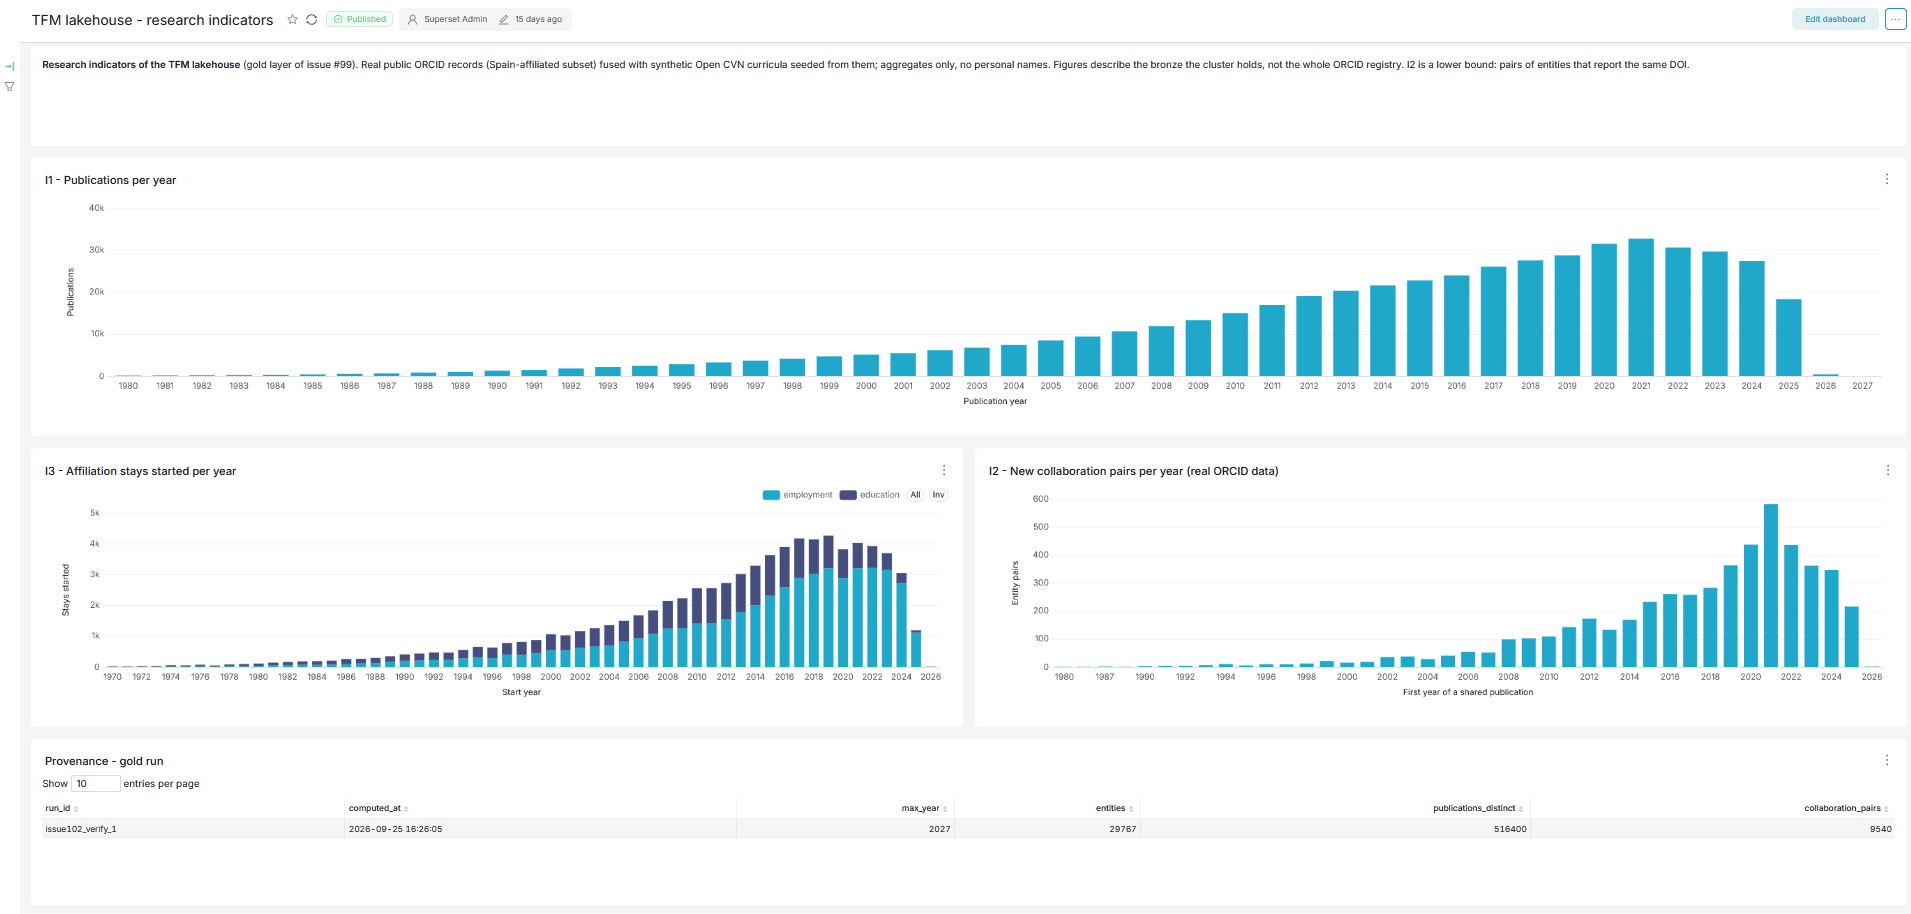
\includegraphics[width=\textwidth]{figs/panel_superset.png}
  \caption{Panel de indicadores de investigación en Apache Superset,
  con los tres indicadores y la tabla de procedencia de la ejecución.}
  \label{fig:tfm_panel_superset}
\end{figure}

La conexión del panel deshabilita además la caché de resultados, para que
una nueva ejecución del flujo de transformación se refleje de inmediato
sin necesidad de vaciarla a mano. Esto se verificó ejecutando el flujo de
transformación completo del Capítulo~\ref{cap:procesamiento} mientras un
proceso externo consultaba el panel de forma repetida. A lo largo de
1\,040 segundos y 238 consultas no se encontró ningún error ni ninguna
respuesta vacía. El identificador de ejecución mostrado por el panel pasó
de la ejecución anterior a la nueva en un único paso, sin ningún estado
intermedio visible, mientras el resto de cifras permanecía igual, como
corresponde a una transformación determinista sobre los mismos datos de
origen.

\section{Metodología y resultados del banco de pruebas de rendimiento}
\label{sec:visualizacion_benchmark}

El banco de pruebas mide el efecto del número de ejecutores de Spark sobre
el tiempo de los tres trabajos de transformación del
Capítulo~\ref{cap:procesamiento}, a tres escalas de volumen de datos y con
tres cantidades de ejecutores en cada una. La campaña se aísla por
completo de los datos de producción, con su propio cubo de MinIO, sus
propios espacios de nombres de Iceberg y su propio esquema de PostgreSQL
por escala, de forma que ninguna medición pueda alterar el panel del
Capítulo~\ref{cap:procesamiento} ni sus propios datos.

Cada combinación de escala y número de ejecutores se ejecuta varias veces.
La primera ejecución de cada escala se descarta como calentamiento, porque
leer un volumen de datos por primera vez resultó sistemáticamente más
lento que las ejecuciones siguientes. Las ejecuciones que sí cuentan se
repiten tres veces, intercaladas entre configuraciones en lugar de
agrupadas, para que una deriva del propio equipo durante la campaña no se
confunda con un efecto del número de ejecutores. La corrección de cada
resultado se comprueba además con una huella de contenido de las tablas
producidas, calculada de forma independiente de su orden. Dos
configuraciones distintas que terminan con éxito sobre la misma escala
deben producir exactamente la misma huella, y así ocurrió en todos los
casos comparables de la campaña.

La captura de estas métricas no necesitó desplegar una pila de
observabilidad dedicada como Prometheus~\cite{prometheus_docs} junto con
Grafana~\cite{grafana_docs}. Cada ejecución de Spark ya escribe su propio
registro de eventos, con la duración de cada etapa y tarea y el uso de
cada ejecutor, y ese registro basta para una campaña acotada como esta.
Instalar y operar una pila de observabilidad continua solo para esta
campaña puntual no estaba justificado, y queda documentada como trabajo
futuro para un despliegue en producción.

El hallazgo principal es que el número de ejecutores no es solo una
palanca de velocidad. A partir de cierto volumen, se convierte en una
palanca de fiabilidad. Con el dimensionamiento de memoria fijo por
ejecutor empleado en esta campaña, un único ejecutor deja de poder
completar el trabajo de validación y normalización de forma determinista
a partir del doble del volumen base, agotando su memoria en cada intento.
A cuádruple volumen, ni siquiera dos ejecutores bastan para ese mismo
trabajo, y solo se completa con cuatro. La Figura~\ref{fig:tfm_benchmark_silver}
muestra este comportamiento sobre el volumen base, donde el trabajo sí
completa a cualquier número de ejecutores.

\begin{figure}[H]
  \centering
  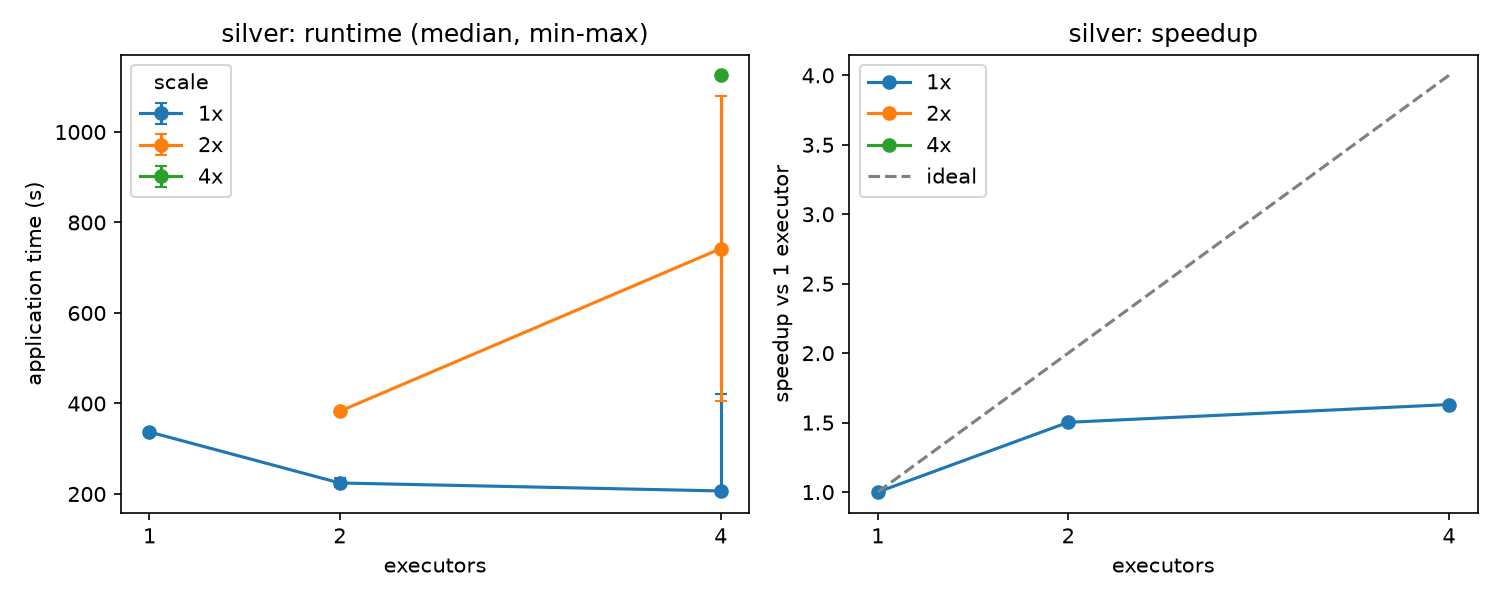
\includegraphics[width=\textwidth]{figs/benchmark_silver.png}
  \caption{Tiempo de ejecución y aceleración del trabajo de validación y
  normalización, sobre el volumen de datos base.}
  \label{fig:tfm_benchmark_silver}
\end{figure}

Incluso cuando el trabajo sí completa, la aceleración queda lejos de la
ideal. Sobre el volumen base, pasar de uno a dos ejecutores da una
aceleración de 1,50, y pasar a cuatro solo sube esa cifra a 1,63, con una
eficiencia que cae de 0,75 a 0,41. Los otros dos trabajos de la
transformación se comportan de forma todavía más marcada. El cálculo de
indicadores ve su eficiencia caer de 1,00 a 0,53 y a 0,23 al pasar de uno
a dos y a cuatro ejecutores, en cualquiera de las tres escalas, porque su
volumen de datos, ya agregado, es demasiado pequeño para aprovechar más
paralelismo. La publicación en PostgreSQL apenas crece con el volumen de
datos en absoluto, con un tiempo de entre 61 y 142 segundos en cualquier
combinación de escala y número de ejecutores, frente a un crecimiento
prácticamente lineal del trabajo de validación con el volumen. La
Tabla~\ref{tab:tfm_benchmark_exponentes} resume esta diferencia mediante
el exponente de la relación entre tiempo y volumen de datos, donde un
valor de 1 indica crecimiento lineal y un valor negativo indica que el
tiempo no depende del volumen.

\begin{table}[H]
  \centering
  \small
  \renewcommand{\arraystretch}{1.2}
  \begin{tabular}{
    >{\raggedright\arraybackslash}p{0.34\textwidth}
    p{0.18\textwidth} p{0.18\textwidth} p{0.18\textwidth}}
    \hline
    \textbf{Trabajo} & \textbf{1 ejecutor} & \textbf{2 ejecutores} & \textbf{4 ejecutores} \\
    \hline
    Validación y normalización & -- & 0,77 & 1,22 \\
    Cálculo de indicadores & 0,97 & 0,96 & 0,79 \\
    Publicación en PostgreSQL & -0,09 & -0,15 & -0,16 \\
    \hline
  \end{tabular}
  \caption{Exponente de crecimiento del tiempo de ejecución frente al
  volumen de datos, por trabajo y número de ejecutores.}
  \label{tab:tfm_benchmark_exponentes}
\end{table}

Ninguna de las tres etapas satura por falta de procesador. El uso de
sistema nunca superó el 32,2\% en ninguna ejecución, y ese máximo se dio
precisamente con cuatro ejecutores, el mismo punto donde el uso del
procesador del propio servicio de almacenamiento de objetos también
alcanzó su máximo. Este patrón apunta al almacenamiento de objetos
compartido, y no al procesador, como el límite más probable de la
plataforma en un único nodo. Esa lectura es consistente con los datos
disponibles, pero no queda demostrada de forma concluyente, ya que el
mecanismo exacto dentro del servicio de almacenamiento no se aisló más
allá de esta medición.

\section{Endurecimiento: fallos operativos reales encontrados y corregidos}
\label{sec:visualizacion_endurecimiento}

A diferencia de las limitaciones de diseño aceptadas de antemano en
capítulos anteriores, esta sección recoge fallos reales que aparecieron
usando el sistema completo bajo condiciones reales, no en una
demostración controlada. Encontrar y corregir un fallo de un componente
externo mediante diagnóstico y una recuperación operativa reproducible es,
en sí mismo, un resultado de este trabajo.

\begin{itemize}
  \item \textbf{Bloqueo permanente del orquestador de flujos.} Tras un
  periodo de funcionamiento sostenido, el propio servidor de tareas de
  Airflow quedó incapaz de arrancar, fallando de la misma forma en cada
  reinicio. La causa es un error conocido, sin corregir todavía en la
  versión de Airflow empleada, que se dispara al reconciliar una tarea
  huérfana cuyo pod ya no existe. El registro de esa tarea concreta
  quedaba almacenado sin marcarse como terminado, así que cada arranque
  del servidor volvía a intentar reconciliarla y volvía a fallar de la
  misma manera. Al tratarse de un error sin corrección disponible en la
  propia herramienta, la solución fue operativa en lugar de un cambio de
  código. Marcar manualmente esa tarea como fallida y reiniciar el
  servidor de tareas resolvió el bloqueo de inmediato. Esta misma
  incidencia volvió a producirse, de forma independiente, semanas
  después, y la misma receta operativa la resolvió de nuevo sin ningún
  cambio adicional.
  \item \textbf{Cierre del servidor de la interfaz de Airflow bajo carga.}
  Ese mismo servidor carecía de una reserva explícita de procesador y
  memoria, lo que le asignaba la prioridad de planificación más baja de
  todo el clúster. Bajo carga del propio nodo, quedaba desatendido el
  tiempo suficiente para que su propia comprobación de salud lo diera por
  bloqueado y lo reiniciase, interrumpiendo cualquier flujo que
  dependiera de él en ese momento. Se corrigió fijando una reserva
  explícita de recursos para ese servidor y relajando los tiempos de su
  comprobación de salud. La corrección se verificó en el propio clúster
  momentos después de que el fallo original volviera a producirse de
  forma independiente, confirmando que el nuevo ajuste resolvía
  exactamente ese mismo patrón.
\end{itemize}

\section{Verificación de extremo a extremo: reconstrucción desde cero}
\label{sec:visualizacion_verificacion}

La plataforma se diseñó para poder reconstruirse desde cero siguiendo
únicamente una guía escrita, sin pasos manuales no documentados. Esa guía
se validó en la práctica y no solo se redactó. La reconstrucción completa
se hizo sobre un clúster Kubernetes aislado y desechable, levantado con
k3d~\cite{k3d_docs}, en lugar de destruir el clúster real que ya contenía
los datos de producción de los capítulos anteriores. El clúster aislado
se configuró con la misma versión exacta de Kubernetes que el clúster
real, y con el propio repositorio de código montado en la misma ruta, de
forma que la guía se siguiera sin ningún paso distinto al que seguiría un
lector cualquiera.

Esta reconstrucción encontró un fallo real no observado hasta entonces.
Al arrancar todos los servicios base a la vez sobre un clúster
completamente nuevo, el primer arranque de PostgreSQL quedó interrumpido
por la contención de arrancar varios servicios a la vez, antes de llegar a
crear el usuario que la capa \textit{gold} necesita. La imagen empleada no
reintenta esa inicialización interrumpida en arranques posteriores, así
que el servicio quedaba disponible pero permanentemente incapaz de
autenticar ese usuario. El fallo se diagnosticó revisando el registro del
propio contenedor y se corrigió forzando una reinicialización completa de
ese servicio. Con esa corrección aplicada, la plataforma completa,
incluidos ambos flujos de Airflow y el panel de Superset con su propio
contenido importado, funcionó de extremo a extremo sobre el clúster
recién creado. El clúster aislado se eliminó al terminar, sin que el
clúster real ni sus datos de producción se vieran afectados en ningún
momento del proceso.


% Conclusiones, competencias y trabajo futuro
% \chapter{Conclusiones, competencias y trabajo futuro}
\label{cap:conclusiones}

El Capítulo~\ref{cap:introduccion} planteó el problema de partida y un
objetivo general acompañado de nueve objetivos específicos. Los capítulos
intermedios han desplegado, capa a capa, la plataforma que responde a ese
planteamiento, y el Capítulo~\ref{cap:visualizacion} ha aportado evidencia
reproducible de su comportamiento. Este capítulo cierra el documento
retomando esos objetivos, relacionando el trabajo con los resultados de
aprendizaje del máster, y señalando las limitaciones y el trabajo futuro
que se derivan de todo lo anterior.

\section{Resumen del trabajo}
\label{sec:conclusiones_resumen}

\textbf{Problema y motivación.} La información curricular y de trayectoria
investigadora está dispersa entre documentos individuales, como CVN, y
registros públicos a escala masiva, como ORCID, sin una plataforma
abierta y autoalojada que combine ambas naturalezas de dato, tal y como se
planteó en el Capítulo~\ref{cap:introduccion}.

\textbf{Arquitectura desplegada.} Este trabajo construye una plataforma
\textit{lakehouse}, justificada en el Capítulo~\ref{cap:estado_arte} y
desplegada en el Capítulo~\ref{cap:infraestructura}: Kubernetes, MinIO con
Iceberg, Spark orquestado por Airflow y PostgreSQL. El
Capítulo~\ref{cap:ingesta} ingiere y fusiona ORCID real y CVN sintético, y
el Capítulo~\ref{cap:procesamiento} resuelve su identidad y calcula los
indicadores.

\textbf{Resultados.} El Capítulo~\ref{cap:visualizacion} publica esos
indicadores en un panel verificado en directo, mide el efecto del
paralelismo sobre el rendimiento, y documenta fallos operativos reales
corregidos, incluida una reconstrucción completa desde cero.

\section{Cumplimiento de los objetivos}
\label{sec:conclusiones_objetivos}

El objetivo general planteado en el Capítulo~\ref{cap:introduccion} era
diseñar, desplegar y evaluar una plataforma que integrase CVN sintético y
ORCID real, los procesase con resolución de identidad entre fuentes, y
publicase indicadores en un panel evaluado mediante un banco de pruebas de
rendimiento. Se considera cumplido. La Tabla~\ref{tab:tfm_conclusiones_objetivos}
detalla cada objetivo específico, en el mismo orden del
Capítulo~\ref{cap:introduccion}.

Uno de los objetivos se cumple con garantías parciales, de forma medida y
no oculta: la integración de ORCID con CVN alcanza una precisión del
95,8\% y una cobertura del 74,2\% en su regla de repliegue por nombre y
afiliación, por debajo del objetivo de precisión fijado antes de medir. El
Capítulo~\ref{cap:procesamiento} explicó por qué perseguirla
artificialmente con más reglas empeoraría, no mejoraría, la fiabilidad del
sistema.

\begin{table}[H]
  \centering
  \small
  \renewcommand{\arraystretch}{1.1}
  \begin{tabular}{
    p{0.08\textwidth}
    >{\raggedright\arraybackslash}p{0.66\textwidth}
    p{0.16\textwidth}}
    \hline
    \textbf{Obj.} & \textbf{Descripción resumida} & \textbf{Cumplimiento} \\
    \hline
    OE1 & Despliegue de la infraestructura base de la plataforma & Cumplido \\
    OE2 & Validación del mecanismo central de almacenamiento y procesamiento & Cumplido \\
    OE3 & Incorporación de datos ORCID reales & Cumplido \\
    OE4 & Incorporación de currículos CVN validados frente a Open CVN & Cumplido \\
    OE5 & Integración de ORCID con CVN por medio de Open CVN & Cumplido con garantías parciales \\
    OE6 & Cálculo y publicación consistente de indicadores & Cumplido \\
    OE7 & Visualización de los indicadores en un panel accesible & Cumplido \\
    OE8 & Banco de pruebas de rendimiento por paralelismo y escala & Cumplido \\
    OE9 & Robustez operativa mediante uso real y guía de reproducción & Cumplido \\
    \hline
  \end{tabular}
  \caption{Grado de cumplimiento de los objetivos específicos.}
  \label{tab:tfm_conclusiones_objetivos}
\end{table}

\section{Contribuciones principales}
\label{sec:conclusiones_contribuciones}

Las contribuciones de este trabajo quedan demostradas, con evidencia
concreta, a lo largo del documento:

\begin{itemize}
  \item \textbf{Plataforma \textit{lakehouse} verificada de extremo a
  extremo}: el Capítulo~\ref{cap:infraestructura} demuestra con dos
  comprobaciones independientes que el mecanismo central de
  almacenamiento y procesamiento funciona antes de construir ningún flujo
  de negocio sobre él.
  \item \textbf{Mecanismo de fusión entre ORCID y CVN diseñado desde el
  origen del dato}: el Capítulo~\ref{cap:ingesta} siembra los currículos
  sintéticos con el identificador ORCID de su semilla real desde su
  propia generación, sin enlazar dos fuentes independientes a posteriori.
  \item \textbf{Resolución de identidad determinista con evidencia
  auditable}: el Capítulo~\ref{cap:procesamiento} fusiona registros de
  fuentes distintas mediante reglas explícitas, cada una con su propia
  evidencia, y mide su precisión y su cobertura.
  \item \textbf{Hallazgo del banco de pruebas de rendimiento}: el
  Capítulo~\ref{cap:visualizacion} demuestra que el número de ejecutores
  de Spark es una palanca de fiabilidad, no solo de velocidad.
  \item \textbf{Guía de reproducibilidad validada por una reconstrucción
  real}: la plataforma se reconstruyó desde cero sobre un clúster aislado
  siguiendo únicamente esa guía, en el Capítulo~\ref{cap:visualizacion}.
\end{itemize}

\section{Resultados de aprendizaje desarrollados}
\label{sec:conclusiones_outcomes}

El Capítulo~\ref{cap:introduccion} identificó seis resultados de
aprendizaje del máster trabajados en este proyecto. La
Tabla~\ref{tab:tfm_conclusiones_outcomes} recoge su evidencia concreta.

\begin{table}[H]
  \centering
  \footnotesize
  \renewcommand{\arraystretch}{1.05}
  \begin{tabular}{
    p{0.1\textwidth}
    >{\raggedright\arraybackslash}p{0.8\textwidth}}
    \hline
    \textbf{Resultado} & \textbf{Evidencia concreta} \\
    \hline
    CN02 & Arquitectura \textit{lakehouse} justificada en el
    Capítulo~\ref{cap:estado_arte}, desplegada en el
    Capítulo~\ref{cap:infraestructura}. \\
    HA01 & Adquisición y generación de fuentes enlazadas por diseño en el
    Capítulo~\ref{cap:ingesta}, fusionadas en el
    Capítulo~\ref{cap:procesamiento}. \\
    HA02 & Procesamiento distribuido del Capítulo~\ref{cap:procesamiento},
    evaluado cuantitativamente en el Capítulo~\ref{cap:visualizacion}. \\
    HA03 & Orquestación de flujos ETL de los
    Capítulos~\ref{cap:infraestructura} y~\ref{cap:procesamiento}, con su
    almacenamiento escalable. \\
    CP01 & Planificación y despliegue de una solución Big Data, de los
    Capítulos~\ref{cap:estado_arte},~\ref{cap:infraestructura}
    y~\ref{cap:visualizacion}. \\
    CP04 & Proyecto profesional original de la plataforma completa,
    evaluada en el Capítulo~\ref{cap:visualizacion} y cerrada aquí. \\
    \hline
  \end{tabular}
  \caption{Resultados de aprendizaje del máster y evidencia concreta de cada uno.}
  \label{tab:tfm_conclusiones_outcomes}
\end{table}

\section{Limitaciones y trabajo futuro}
\label{sec:conclusiones_limitaciones}

Los capítulos anteriores han documentado limitaciones concretas sin
ocultarlas, distinguiendo las que proceden de un componente de terceros de
las que son una decisión deliberada de alcance. Esta sección las
consolida junto con el trabajo futuro que se deriva de cada una.

La única de origen externo es el \textbf{fallo conocido del orquestador de
flujos}, sin corrección oficial disponible, documentado con su receta
operativa de recuperación en el Capítulo~\ref{cap:visualizacion}. El
trabajo futuro solo puede consistir en incorporar la corrección oficial
cuando exista.

El resto son decisiones deliberadas de alcance, cada una ya justificada en
su capítulo:

\begin{itemize}
  \sloppy
  \item sin capa de consulta interactiva independiente como
  Trino~\cite{trino_docs}
  \item sin observabilidad centralizada como Prometheus~\cite{prometheus_docs}
  y Grafana~\cite{grafana_docs}
  \item un único nodo local, sin infraestructura como código mediante
  Terraform~\cite{terraform_docs}, en vez de un clúster real en la nube
  \item reconstrucción completa de silver y gold en cada ejecución, en
  lugar de procesamiento incremental
  \item resolución de identidad determinista, frente a las alternativas
  probabilísticas ya citadas en el Capítulo~\ref{cap:procesamiento}
\end{itemize}

La Tabla~\ref{tab:tfm_conclusiones_limitaciones} consolida cada una con su
trabajo futuro asociado.

\begin{table}[H]
  \centering
  \footnotesize
  \renewcommand{\arraystretch}{1.0}
  \begin{tabular}{
    >{\raggedright\arraybackslash}p{0.44\textwidth}
    >{\raggedright\arraybackslash}p{0.44\textwidth}}
    \hline
    \textbf{Limitación} & \textbf{Trabajo futuro asociado} \\
    \hline
    Fallo del orquestador de flujos, sin corrección oficial & Incorporar la corrección oficial cuando esté disponible \\
    Sin capa de consulta interactiva independiente & Incorporar un motor de consulta federado si surge esa necesidad \\
    Sin observabilidad centralizada & Desplegar una pila de observabilidad continua para producción \\
    Único nodo local, sin infraestructura como código para la nube & Automatizar el despliegue en la nube sobre la misma definición \\
    Reconstrucción completa en cada ejecución & Procesar de forma incremental sobre los \textit{snapshots} de Iceberg \\
    Resolución de identidad determinista, sin aprendizaje automático & Explorar vinculación probabilística o basada en aprendizaje automático \\
    \hline
  \end{tabular}
  \caption{Limitaciones documentadas y trabajo futuro asociado.}
  \label{tab:tfm_conclusiones_limitaciones}
\end{table}

\section{Conclusiones}
\label{sec:conclusiones_finales}

El resumen, el cumplimiento de objetivos y las contribuciones ya
presentados permiten cerrar el documento con una valoración conjunta. El
objetivo general se considera cumplido y, con él, los nueve objetivos
específicos, con la única salvedad medida de la cobertura de la
resolución de identidad, una limitación de evidencia y no una afirmación
sin respaldo. Las limitaciones recogidas no comprometen esta conclusión.
Delimitan, con precisión y sin ocultamiento, hasta dónde llega la
propuesta actual. Algunas son ajenas al sistema desarrollado y otras son
decisiones deliberadas de alcance, propias de un Trabajo Fin de Máster y
no de un producto cerrado, y el sistema las documenta en lugar de
disimularlas.

En conjunto, este trabajo demuestra que es posible construir, a partir de
CVN y ORCID, una plataforma \textit{lakehouse} autoalojada que fusiona
información curricular documental con registros públicos a escala masiva,
conserva procedencia verificable en cada capa, y ofrece garantías
reproducibles allí donde el proceso es determinista. Esa plataforma
completa, más que el panel de indicadores o cualquier componente aislado
que la demuestra, es la aportación principal de este Trabajo Fin de
Máster.


% Capítulos pendientes de redacción.
% Se incorporarán cuando su contenido esté preparado.

% -------------------------------
% Apéndices
% -------------------------------
% \appendix
% Pendientes de definir; se incorporarán, si procede, cuando el contenido
% principal esté redactado y se sepa qué material de referencia conviene
% mover fuera del cuerpo principal.

\cleardoublepage
\thispagestyle{empty}


% -------------------------------
% Bibliografía
% -------------------------------
\bibliographystyle{apalike}
\bibliography{bib/ref} 
\addcontentsline{toc}{chapter}{Referencia bibliográfica} % Añade a la tabla de contenidos

\end{document}